%%
%% abtex2-modelo-trabalho-academico.tex, v-1.9.2 laurocesar
%% Copyright 2012-2017 by abnTeX2 group at http://abntex2.googlecode.com/ 
%%
%% This work may be distributed and/or modified under the
%% conditions of the LaTeX Project Public License, either version 1.3
%% of this license or (at your option) any later version.
%% The latest version of this license is in
%%   http://www.latex-project.org/lppl.txt
%% and version 1.3 or later is part of all distributions of LaTeX
%% version 2005/12/01 or later.
%%
%% This work has the LPPL maintenance status `maintained'.
%% 
%% The Current Maintainer of this work is Emílio Eiji Kavamura,
%% eek.edu@outlook.com; emilio.kavamura@ufpr.br
%% Further information about abnTeX2 are available on 
%%
%% http://abntex2.googlecode.com/
%%
%% https://code.google.com/p/abntex2/issues/ 
%%
%% Further information about UFPR abnTeX2 are available on 
%%
%% https://github.com/eekBR/ufpr-abntex/
%%
%% This work consists of the files 
% 
%          main.tex   programa principal
%      00-dados.tex   entrada de dados 
%    00-pacotes.tex   pacotes carregados no modelo
% 00-pretextual.tex   processamento dos elementos pre-textuais
%          UFPR.sty   ajusta do modelo canonico às normas  UFPR
%
%    referencias.bib
%                     e outras arquivos de imagens
%
%
%------------------------------------------------------------------------
% ------------------------------------------------------------------------
% abnTeX2: Modelo de Trabalho Academico (tese de doutorado, dissertacao de
% mestrado e trabalhos monograficos em geral) em conformidade com 
% ABNT NBR 6023:2018: Informação e documentação - Referências - Elaboração
% ------------------------------------------------------------------------
% ------------------------------------------------------------------------
%
% DATA DE ATUALIZAÇÃO: 2020-06-10

\documentclass[
        % -- opções da classe memoir --
        12pt,                           % tamanho da fonte
        openright,                      % capítulos começam em pág ímpar (insere página vazia caso preciso)
        %twoside,                        % para impressão em verso e anverso. Oposto a oneside
        oneside,
        a4paper,                        % tamanho do papel. 
        % -- opções da classe abntex2 --
        chapter=TITLE,         % títulos de capítulos convertidos em letras maiúsculas
        section=TITLE,         % títulos de seções convertidos em letras maiúsculas
        subsection=Title,      % títulos de subseções convertidos em letras maiúsculas
        %subsubsection=TITLE,  % títulos de subsubseções convertidos em letras maiúsculas
        % -- opções do pacote babel --
        english,                        % idioma adicional para hifenização
        %french,                         % idioma adicional para hifenização
        spanish,                        % idioma adicional para hifenização
        portugues,                      % o último idioma é o principal do documento
        %%%%%%%%%%%%
        %eek: colocação da opção para o sumario ter formatação tradicional
        %sumario=tradicional             % título no formato tradicional
        ]{abntex2}

\usepackage{UFPR}
% Pacotes básicos 
% ----------------------------------------------------------
\usepackage{newtxtext,newtxmath}
		% Usa a fonte Latin Modern			
\usepackage[T1]{fontenc}		% Selecao de codigos de fonte.
\usepackage[utf8]{inputenc}		% Codificacao do documento (conversão automática dos acentos)
\usepackage{lastpage}			% Usado pela Ficha catalográfica
\usepackage{indentfirst}		% Indenta o primeiro parágrafo de cada seção.
\usepackage{color}		    	% Controle das cores
\usepackage{graphicx}			% Inclusão de gráficos
\usepackage{microtype} 			% para melhorias de justificação
\usepackage{ifthen}		    	% para montar condicionais
\usepackage[brazil]{babel}		% para utilizar termos em portugues
\usepackage[final]{pdfpages}    % para incluir páginas de arquivos pdf
\usepackage{lipsum}				% para geração de dummy text
\usepackage{csquotes}

\usepackage{pdflscape}
\usepackage{longtable}
\usepackage{caption}
\usepackage{subcaption}
\usepackage{verbatim}
\usepackage{float}

%\usepackage[style=long]{glossaries}
%\usepackage{abntex2glossaries}


\usepackage{cancel} 		% permite representar o cancelamento de termos em texto ou equacoes	
\usepackage{xcolor} 		% cores extendidas	
\usepackage{smartdiagram}   	% gera diagramas a partir de listas
%\usepackage{float} 		% Para a figura ficar na posição correta	    
\usepackage{textcomp} 		% supporte para fontes da Text Companion 
\usepackage{longtable}		% uso de longtable
\usepackage{amsmath}		% simbolos matematicos
\usepackage{lscape}		% páginas em paisagem
\usepackage{multicol}		% mescla de colunas em tabelas
\usepackage{multirow}		% mescla de linhas em tabelas
\usepackage{newfloat} 		% criação do indice de quadros
%\usepackage{caption} 		% configura legenda 
	%[format=plain]
	%\renewcommand\caption[1]{%
    	%\captionsetup{font=small}	% tamanho da fonte 10pt
    	%,format=hang
 	% \caption{#1}}
	%\captionsetup{width=0.8\textwidth}
\captiondelim{-- }
\captiontitlefont{\small}
\captionnamefont{\small}

% Pacotes de citações BibLaTeX
% ----------------------------------------------------------
\usepackage[style=abnt,
	backref=true,
	backend=biber,
	citecounter=false,
	backrefstyle=three, 
	url=true,
	maxbibnames=99,
    mincitenames=1,
    maxcitenames=2,
    backref=false,
    hyperref=true,
    giveninits=true,
    uniquename=false,
    uniquelist=false]{biblatex}

% Norma NBR10.520/2023 - Sobrenomes em minúsculas
\renewcommand*{\mkbibnamefamily}[1]{#1}%

% Espaçamento entre os itens nas referências (espço de uma linha simples)
% ----------------------------------------------------------
\setlength\bibitemsep{\baselineskip}

% Texto padrão para as referências
% ----------------------------------------------------------
\DefineBibliographyStrings{brazil}{%
	 backrefpage  = {Citado \arabic{citecounter} vez na página},		% originally "cited on page"
	 backrefpages = {Citado \arabic{citecounter} vezes nas páginas},	% originally "cited on pages"
	 urlfrom      = {Dispon\'ivel em},
}

% Ajusta indentação de Referencias no ToC
% ----------------------------------------------------------
\defbibheading{bay}[\bibname]{%
  \chapter*{#1}%
  \markboth{#1}{#1}%
  \addcontentsline{toc}{chapter}
  %{\protect\numberline{}\bibname}
  {\bibname}
}

% Formatando o avançao dos títulos no sumário 
% ----------------------------------------------------------
\makeatletter
	\pretocmd{\chapter}{\addtocontents{toc}{\protect\addvspace{-12\p@}}}{}{}
	\pretocmd{\section}{\addtocontents{toc}{\protect\addvspace{-3\p@}}}{}{}
\makeatother

% https://groups.google.com/g/abntex2/c/ZYwE4t9uTFM
\makeatletter
\let\oldcontentsline\contentsline
\def\contentsline#1#2{%
	\expandafter\ifx\csname l@#1\endcsname\l@section
	\expandafter\@firstoftwo
	\else
	\expandafter\@secondoftwo
	\fi
	{%
		\oldcontentsline{#1}{\MakeTextUppercase{#2}}%
	}{%
		\oldcontentsline{#1}{#2}%
	}%
}
\makeatother

% Para retirar os símbolos <> da URL  
% ----------------------------------------------------------
\DeclareFieldFormat{illustrated}{\addspace #1\isdot}%
%\DeclareFieldFormat{url}{\bibstring{urlform}\addcolon\addspace<\url{#1}>}%
%\DeclareFieldFormat{url}{\bibstring{urlfrom}\addcolon\addspace<\url{#1}>}%
\DeclareFieldFormat{url}{\bibstring{urlfrom}\addcolon \space\addspace{#1}} 
% remove <> em urls de acordo com abnt-6023:2018	

% Ajustar o espaço para a formatação da data
% ----------------------------------------------------------
\DeclareFieldFormat{urldate}{\bibstring{urlseen}\addcolon\addspace #1}%
\DeclareFieldFormat*{note}{\addspace #1}%

% Para ajustar o tamanho da fonte do número da primeira página do capítulo
% comando utilizado na parte textual 
% ----------------------------------------------------------
\makepagestyle{chapfirst}% Just for the first page of a chapter
\makeoddhead{chapfirst}{}{}{\footnotesize{\thepage}}

%%criar um novo estilo de cabeçalhos e rodapés
\makepagestyle{simplestextual}
  %%cabeçalhos
  \makeevenhead{simplestextual} %%pagina par
     {}{}{\footnotesize \thepage}
     
  \makeoddhead{simplestextual} %%pagina ímpar ou com oneside
     {}{}{\footnotesize \thepage}
  %\makeheadrule{simplestextual}{\textwidth}{\normalrulethickness} %linha
  %% rodapé
  \makeevenfoot{simplestextual}
     {}{}{} %%pagina par
      
  \makeoddfoot{simplestextual} %%pagina ímpar ou com oneside
     {}{}{}
     
% Define a formatação dos capítulos póstextuais numerados
% ----------------------------------------------------------
%\newcommand{\refap}[1]{\hyperref[#1]{Apêndice~\ref{#1}}} 	% Referência apÊndices

% uso do tikz e pgfplots
% ----------------------------------------------------------
%\usetikzlibrary{external}
\usetikzlibrary{arrows,calc,patterns,angles,quotes}
\usepackage{pgfplots}
\pgfplotsset{compat=1.15}

% Define o comando para citação de fontes em elementos gráficos (figuras, imagens,...).
% ----------------------------------------------------------
%  AUTOR(ano)
%
% parâmetro é a bibkey da fonte
  
\newcommand{\citefig}[2]{~\Citeauthor*{#1}\citeyear{#1}}

% Define os operadores matemáticos em portugues
% ----------------------------------------------------------
%

\DeclareMathOperator{\tr}{tr}
\DeclareMathOperator{\sen}{sen}
\DeclareMathOperator{\senh}{senh}
%\DeclareMathOperator{\tag}{tag}
\DeclareMathOperator{\tg}{tg}
\DeclareMathOperator{\tagh}{tagh}
\DeclareMathOperator{\tgh}{tgh}
\DeclareMathOperator{\cossec}{cossec}
%\DeclareMathOperator{\sen}{sen}

% Para fazer a listagem de codigos LaTeX na documentação
% ----------------------------------------------------------
\usepackage{listings}

% Comando para fazer 
%    a citação de documentos não publicados e informais e 
%    colocar as referências nas notas de rodapé
% ----------------------------------------------------------

\newcommand{\citenp}[1]{
\cite{#1}\footnote{\fullcite{#1}}}

\newcommand{\textcitenp}[1]{
	\textcite{#1}\footnote{\fullcite{#1}}}

 %%%%%%%%%%% NBR 10520/23

 % Norma NBR10.520/2023 - Sobrenomes em minúsculas
\renewcommand*{\mkbibnamefamily}[1]{#1}%

%fullcite com todos autores e não como cite
\makeatletter
\newcommand{\tempmaxup}[1]{\def\blx@maxcitenames{99}#1}
\makeatother

\DeclareCiteCommand{\fullcite}[\tempmaxup]
{\usebibmacro{prenote}}
{\usedriver
	{}
	{\thefield{entrytype}}}
{\multicitedelim}
{\usebibmacro{postnote}}

\usepackage{pdflscape}
\usepackage{longtable}
\usepackage{caption}
\usepackage{subcaption}
\usepackage{verbatim}
\usepackage{tabularray}
\usepackage{float}
\usepackage{graphicx}
\usepackage{codehigh}
\usepackage[normalem]{ulem}
\UseTblrLibrary{booktabs}
\UseTblrLibrary{siunitx}
\newcommand{\tinytableTabularrayUnderline}[1]{\underline{#1}}
\newcommand{\tinytableTabularrayStrikeout}[1]{\sout{#1}}
\NewTableCommand{\tinytableDefineColor}[3]{\definecolor{#1}{#2}{#3}}


%%%%%%%%%%%%%%%%%%%%%%%%%%%%%%%%%%%%%%%%%%%%%%%%%%%%%%%
% Arquivo para entrada de dados para a parte pré textual
%%%%%%%%%%%%%%%%%%%%%%%%%%%%%%%%%%%%%%%%%%%%%%%%%%%%%%%
% 
% Basta digitar as informações indicidas, no formato 
% apresentado.
%
%%%%%%%
% Os dados solicitados são, na ordem:
%
% tipo do trabalho
% componentes do trabalho 
% título do trabalho
% nome do autor
% local 
% data (ano com 4 dígitos)
% orientador(a)
% coorientador(a)(as)(es)
% arquivo com dados bibliográficos
% instituição
% setor
% programa de pós gradução
% curso
% preambulo
% data defesa
% CDU
% errata
% assinaturas - termo de aprovação
% resumos & palavras chave
% agradecimentos
% dedicatoria
% epígrafe


% Informações de dados para CAPA e FOLHA DE ROSTO
%----------------------------------------------------------------------------- 
\tipotrabalho{Trabalho de Conclusão de Curso}
%    {Relatório Técnico}
%    {Dissertação}
%    {Tese}
%    {Monografia}

% Marcar Sim para as partes que irão compor o documento pdf
%----------------------------------------------------------------------------- 
 \providecommand{\terCapa}{Sim}
 \providecommand{\terFolhaRosto}{Sim}
 \providecommand{\terTermoAprovacao}{Sim}
 \providecommand{\terDedicatoria}{Nao}
 \providecommand{\terFichaCatalografica}{Sim}
 \providecommand{\terEpigrafe}{Nao}
 \providecommand{\terAgradecimentos}{Sim}
 \providecommand{\terErrata}{Nao}
 \providecommand{\terListaFiguras}{Sim}
 \providecommand{\terListaQuadros}{Nao}
 \providecommand{\terListaTabelas}{Sim}
 \providecommand{\terSiglasAbrev}{Nao} 
 \providecommand{\terSimbolos}{Nao}
 \providecommand{\terResumos}{Sim}
 \providecommand{\terSumario}{Sim}
 \providecommand{\terAnexo}{Nao}
 \providecommand{\terApendice}{Sim}
 \providecommand{\terIndiceR}{Nao}
%----------------------------------------------------------------------------- 

\titulo{Mais Que Uma Sala de Aula: O Impacto do Ensino Médio Integral Sobre Resultados Escolares Brasileiros}
\autor{Victor Manoel Alves}
\local{São Paulo - SP}
\data{2024} %Apenas ano 4 dígitos

% Orientador ou Orientadora
\orientador{}
%Prof Emílio Eiji Kavamura, MSc}
\orientadora{
Cristine Campos de Xavier Pinto}
% Pode haver apenas uma orientadora ou um orientador
% Se houver os dois prevalece o feminino.

% Em termos de coorientação, podem haver até quatro neste modelo
% Sendo 2 mulhere e 2 homens.
% Coorientador ou Coorientadora
\coorientador{}%Prof Morgan Freeman, DSc}
\coorientadora{}

% Segundo Coorientador ou Segunda Coorientadora
\scoorientador{}
%Prof Jack Nicholson, DEng}
\scoorientadora{}
%Prof\textordfeminine~Ingrid Bergman, DEng}
% ----------------------------------------------------------
\addbibresource{referencias.bib}

% ----------------------------------------------------------
\instituicao{%
Insper Instituto de Ensino e Pesquisa}

\def \ImprimirSetor{}%
%Setor de Tecnologia}

\def \ImprimirProgramaPos{}%Programa de Pós Graduação em Engenharia de Construção Civil}

\def \ImprimirCurso{}
%Curso de Engenharia Civil}

\preambulo{
Monografia apresentada ao programa de Graduação Em Economia como requisito para obtenção do rótulo de Bacharel em economia.}
%do grau de Bacharel em Expressão Gráfica no curso de Expressão Gráfica, Setor de Exatas da Universidade Federal do Paraná}

%----------------------------------------------------------------------------- 

\newcommand{\imprimirCurso}{Economia}
%Programa de P\'os Gradua\c{c}\~ao em Engenharia da Constru\c{c}\~ao Civil}

\newcommand{\imprimirDataDefesa}{
09 de Dezembro de 2018}

\newcommand{\imprimircdu}{
02:141:005.7}

% ----------------------------------------------------------
\newcommand{\imprimirerrata}{
Elemento opcional da \cites[4.2.1.2]{NBR14724:2011}. Exemplo:

\vspace{\onelineskip}

FERRIGNO, C. R. A. \textbf{Tratamento de neoplasias ósseas apendiculares com
reimplantação de enxerto ósseo autólogo autoclavado associado ao plasma
rico em plaquetas}: estudo crítico na cirurgia de preservação de membro em
cães. 2011. 128 f. Tese (Livre-Docência) - Faculdade de Medicina Veterinária e
Zootecnia, Universidade de São Paulo, São Paulo, 2011.

\begin{table}[htb]
\center
\footnotesize
\begin{tabular}{|p{1.4cm}|p{1cm}|p{3cm}|p{3cm}|}
  \hline
   \textbf{Folha} & \textbf{Linha}  & \textbf{Onde se lê}  & \textbf{Leia-se}  \\
    \hline
    1 & 10 & auto-conclavo & autoconclavo\\
   \hline
\end{tabular}
\end{table}}

% Comandos de dados - Data da apresentação
\providecommand{\imprimirdataapresentacaoRotulo}{}
\providecommand{\imprimirdataapresentacao}{}
\newcommand{\dataapresentacao}[2][\dataapresentacaoname]{\renewcommand{\dataapresentacao}{#2}}

% Comandos de dados - Nome do Curso
\providecommand{\imprimirnomedocursoRotulo}{}
\providecommand{\imprimirnomedocurso}{}
\newcommand{\nomedocurso}[2][\nomedocursoname]
  {\renewcommand{\imprimirnomedocursoRotulo}{#1}
\renewcommand{\imprimirnomedocurso}{#2}}


% ----------------------------------------------------------
\newcommand{\AssinaAprovacao}{

\assinatura{%\textbf
   {Naercio Aquino Menezes Filho \\ Insper}}
      
   \begin{center}
    \vspace*{0.5cm}
    %{\large\imprimirlocal}
    %\par
    %{\large\imprimirdata}
    \imprimirlocal\\
    2024
    \vspace*{1cm}
  \end{center}
  }
  
% ----------------------------------------------------------
%\newcommand{\Errata}{%\color{blue}
%Elemento opcional da \textcite[4.2.1.2]{NBR14724:2011}. Exemplo:
%}

% ----------------------------------------------------------
\newcommand{\EpigrafeTexto}{%\color{blue}
\textit{``Não vos amoldeis às estruturas deste mundo, \\
		mas transformai-vos pela renovação da mente, \\
		a fim de distinguir qual é a vontade de Deus: \\
		o que é bom, o que Lhe é agradável, o que é perfeito.\\
		(Bíblia Sagrada, Romanos 12, 2)}
}

% ----------------------------------------------------------
\newcommand{\ResumoTexto}{%\color{blue}
    Este trabalho de conclusão de curso explora os efeitos da ampliação da jornada escolar sobre o desempenho acadêmico dos alunos. A pesquisa investiga como o aumento do tempo de permanência dos alunos na escola afeta seu desempenho em testes padronizados e em indicadores educacionais selecionados. A análise é realizada com base em uma revisão abrangente da literatura global e evidências específicas para o contexto brasileiro. Para obtenção do efeito causal do programa Ensino Médio Integral sobre alunos brasileiros, adota-se a metodologia de \textit{staggered difference-in-differences} sobre dados públicos do Instituto Nacional de Estudos e Pesquisas Educacionais Anísio Teixeira, ainda não aplicada para avaliar o programa a nível nacional. Os resultados sugerem melhoras ao longo do tempo de exposição sobre as notas dos alunos nas provas do Exame Nacional do Ensino Médio de escolas participantes. Os resultados também apontam para melhoras nas taxas de abandono e aprovação para escolas participantes.} 

\newcommand{\PalavraschaveTexto}{%\color{blue}
Programa Ensino Médio Integral, Desempenho Acadêmico, \textit{Staggered difference-In-differences}.}

% ----------------------------------------------------------
\newcommand{\AbstractTexto}{%\color{blue}
This undergraduate thesis explores the effects of extending the school day on students' academic performance. The research investigates how increasing students' time spent in school affects their performance on standardized tests and selected educational indicators. The analysis is based on a comprehensive review of global literature and evidence specific to the Brazilian context. To obtain the causal effect of the Full High School program on Brazilian students, the methodology of staggered difference-in-differences is adopted using publicly available data from the Instituto Nacional de Estudos e Pesquisas Educacionais Anísio Teixeira, which has not yet been applied to evaluate the program at the national level. The results suggest improvements over time in students' scores on the Exame Nacional do Ensino Médio for participating schools. There are also improvements in dropout rates and approval rates for participating schools.
}
% ---
\newcommand{\KeywordsTexto}{%\color{blue}
Full-Time High School Program, Academic Performance, Staggered difference-in-differences.
}

% ----------------------------------------------------------
\newcommand{\Resume}
{%\color{blue}
%Il s'agit d'un résumé en français.
} 
% ---
\newcommand{\Motscles}
{%\color{blue}
 %latex. abntex. publication de textes.
}

% ----------------------------------------------------------
\newcommand{\Resumen}
{%\color{blue}
%Este es el resumen en español.
}
% ---
\newcommand{\Palabrasclave}
{%\color{blue}
%latex. abntex. publicación de textos.
}

% ----------------------------------------------------------
\newcommand{\AgradecimentosTexto}{%\color{blue}

Expresso minha sincera gratidão à minha avó, Maria, e à minha mãe, Cristiane, pelo sacrifício e apoio incansável que tornaram possível minha jornada até este ponto. À minha querida irmã, Vitória, agradeço pela presença constante e pelo apoio inestimável ao longo desta trajetória.

A Deus e aos orixás pela proteção e resiliência que me permitiram trilhar esta jornada.

Aos membros do grupo Green Bay ANPECkers, meu sincero obrigado por nossa jornada conjunta. Aos amigos de escola e ao meu irmão de vida, Paulo, agradeço pela colaboração e pelo sucesso que alcançamos juntos. Um agradecimento especial à Ana Flavia pelo seu constante companheirismo.

A todos os mentores que encontrei ao longo de minha trajetória acadêmica e profissional. Cristine, Thiago, Ricardo, Adriano, Davi e Thais, é um privilégio ter vocês como inspiração de profissional que desejo ser. E ao Programa de Bolsas, agradeço por acreditar em meu potencial e por proporcionar a oportunidade incrível e altamente impactante que vivenciei aqui.
}

% ----------------------------------------------------------
\newcommand{\DedicatoriaTexto}{%\color{blue}
\textit{ Este trabalho é dedicado às crianças adultas que,\\
   quando pequenas, sonharam em se tornar cientistas.}
	}



% compila o indice
% 
% ----------------------------------------------------------


\makeindex
% ----------------------------------------------------------
% Início do documento
% ----------------------------------------------------------
\begin{document}
% ----------------------------------------------------------
% Adequando o uppercase titulo dos elementos nas suas respectivas legendas
% Definicoes que n\~ao funcionaram quando colocados no arquivo de estilos ou de pacotes

\renewcommand{\bibname}{{REFER\^ENCIAS}}
\renewcommand{\tablename}{Tabela }
\renewcommand{\figurename}{Figura }
\renewcommand{\figureautorefname}{Figura}
\renewcommand{\tableautorefname}{Tabela}
\newcommand{\equationname}{Equa\c{c}\~ao~}
\renewcommand{\equationautorefname}{Equa\c{c}\~ao~}

% Para ajustar o tamanho da fonte do número da primeira página do capítulo
\aliaspagestyle{chapter}{chapfirst}% customizing chapter pagestyle

% ELEMENTOS PRÉ-TEXTUAIS
\makeoddhead{chapfirst}{}{}{}
% ----------------------------------------------------------
% Capa
% ----------------------------------------------------------
 \ifthenelse{\equal{\terCapa}{Sim}}{
\imprimircapa}{}

% Folha de rosto
% ----------------------------------------------------------
\imprimirfolhaderosto*

% Inserir a ficha bibliografica
% ----------------------------------------------------------
 \ifthenelse{\equal{\terFichaCatalografica}{Sim}}
 {\insereFichaCatalografica{}\cleardoublepage}
 {}

% Inserir errata
% ----------------------------------------------------------
 \ifthenelse{\equal{\terErrata}{Sim}}
 {\begin{errata}%\color{blue}
   \imprimirerrata
  \end{errata}}
 {}

% Inserir folha de aprovação
% ----------------------------------------------------------
\ifthenelse{\equal{\terTermoAprovacao}{Sim}}{
\insereAprovacao}{}

% Dedicatória
% ----------------------------------------------------------
\ifthenelse{\equal{\terDedicatoria}{Sim}}{
\begin{dedicatoria}
   \vspace*{\fill}
   \centering
   \noindent
   \DedicatoriaTexto
   \vspace*{\fill}
\end{dedicatoria}
}{}

% Agradecimentos
% ----------------------------------------------------------

 \ifthenelse{\equal{\terAgradecimentos}{Sim}}
 {\begin{agradecimentos}
    \AgradecimentosTexto
  \end{agradecimentos}
  }{}
% Epígrafe
% ----------------------------------------------------------

\ifthenelse{\equal{\terEpigrafe}{Sim}}{
\begin{epigrafe}
    \vspace*{\fill}
	\begin{flushright}
        \EpigrafeTexto
	\end{flushright}
\end{epigrafe}
}{}

% RESUMOS
% ----------------------------------------------------------
% resumo em português
%\setlength{\absparsep}{18pt} % ajusta o espaçamento dos parágrafos do resumo
 \ifthenelse{\equal{\terResumos}{Sim}}{
\begin{resumo}
    \ResumoTexto

    
    \textbf{Palavras-chaves}:  \PalavraschaveTexto
\end{resumo}

%% resumo em inglês
\begin{resumo}[ABSTRACT]
 \begin{otherlanguage*}{english}
   \AbstractTexto

   %\vspace{\onelineskip}
   \noindent 
   \textbf{Key-words}: 
 \KeywordsTexto
 \end{otherlanguage*}
\end{resumo}


% resumo em francês 
\ifthenelse{\equal{\Resume}{}}
{}
{
 \begin{resumo}[RESUME]%Résumé
  \begin{otherlanguage*}{french}
     \Resume
     
     %\vspace{\onelineskip}
     \noindent      
     \textbf{Mots clés}: \Motscles
  \end{otherlanguage*}
 \end{resumo}
} 

% resumo em espanhol
\ifthenelse{\equal{\Resume}{}}{}
{ \begin{resumo}[RESUMEN]
  \begin{otherlanguage*}{spanish}
    \Resumen 
   
   %\vspace{\onelineskip}
   \noindent    
    \textbf{Palabras clave}: \Palabrasclave
  \end{otherlanguage*}
 \end{resumo}
}
}{}

% inserir lista de ilustrações
% ----------------------------------------------------------
\ifthenelse{\equal{\terListaFiguras}{Sim}}{
%\pdfbookmark[0]{\listfigurename}{lof}
\listoffigures*
\cleardoublepage
}{}

% inserir lista de quadros
% ----------------------------------------------------------
\ifthenelse{\equal{\terListaQuadros}{Sim}}{
%\pdfbookmark[0]{\listtablename}{lot}
\listofquadros*
\cleardoublepage
}{}

% inserir lista de tabelas
% ----------------------------------------------------------
\ifthenelse{\equal{\terListaTabelas}{Sim}}{
%\pdfbookmark[0]{\listtablename}{lot}
\listoftables*
\cleardoublepage
}{}



% inserir lista de abreviaturas e siglas 
% ----------------------------------------------------------

 \ifthenelse{\equal{\terSiglasAbrev}{Sim}}{
    \imprimirlistadesiglas
    \cleardoublepage
}{}


% inserir lista de símbolos
% ----------------------------------------------------------

 \ifthenelse{\equal{\terSimbolos}{Sim}}{
    \imprimirlistadesimbolos
    \cleardoublepage
 }{}

% inserir o sumario
\makeoddhead{chapfirst}{}{}{}
% ----------------------------------------------------------
\ifthenelse{\equal{\terSumario}{Sim}}{
\pdfbookmark[0]{\contentsname}{toc}
\pagestyle{empty}
\tableofcontents*
\thispagestyle{empty}
\cleardoublepage
}{}
 

 
 


% ----------------------------------------------------------
% ELEMENTOS TEXTUAIS
% ----------------------------------------------------------
\textual % \pagestyle{textualUFPR}

\pagestyle{simplestextual}
% sugerido por Youssef Cherem 20170316
% https://mail.google.com/mail/u/0/?tab=wm#inbox/15ad3fe6f4e5ff1f

% Introdução (exemplo de capítulo sem numeração, mas presente no Sumário)
% ----------------------------------------------------------
% ---------------------------  Introdução ------------------------------- %
\chapter{Introdução}

O Plano Nacional de Educação estabelece a seguinte meta: "Oferecer educação em tempo integral em, no mínimo, 50\% das escolas públicas, atendendo, pelo menos, 25\% dos alunos da educação básica." Essa meta reflete a visão da escola não apenas como um local de aprendizado acadêmico, mas como uma instituição que molda cidadãos para o mundo.

 Os dados do Instituto Nacional de Estudos e Pesquisas Educacionais Anísio Teixeira (INEP) indicam um aumento no acesso à educação entre jovens e adolescentes. Se olharmos para os dados de aprovação é perceptível uma melhora ao longo dos anos da série, sendo ela cerca de 76\% em 2007 e 86\% em 2022 para alunos do ensino médio.

Quando olhando para o desempenho dos estudantes do Brasil o cenário não é favorável. De acordo com o Program for International Student Assessment (PISA), que compara o desempenho de estudantes em nível internacional, os alunos brasileiros estão aquém da média dos estudantes de países participantes da OCDE desde o início da aplicação dos testes no ano de 2000. A nível nacional, o Índice de Desenvolvimento da Educação Básica (IDEB) aponta que o desempenho médio no ensino fundamental está abaixo do necessário para se equiparar aos países com alta qualidade educacional. Ademais, quando olhamos para as notas obtidas no Exame Nacional do Ensino Médio (ENEM) vemos notas baixas em relação à escala de notas possíveis.

\begin{figure}[H]
    \centering
    \caption{Evolução de notas do ENEM}
    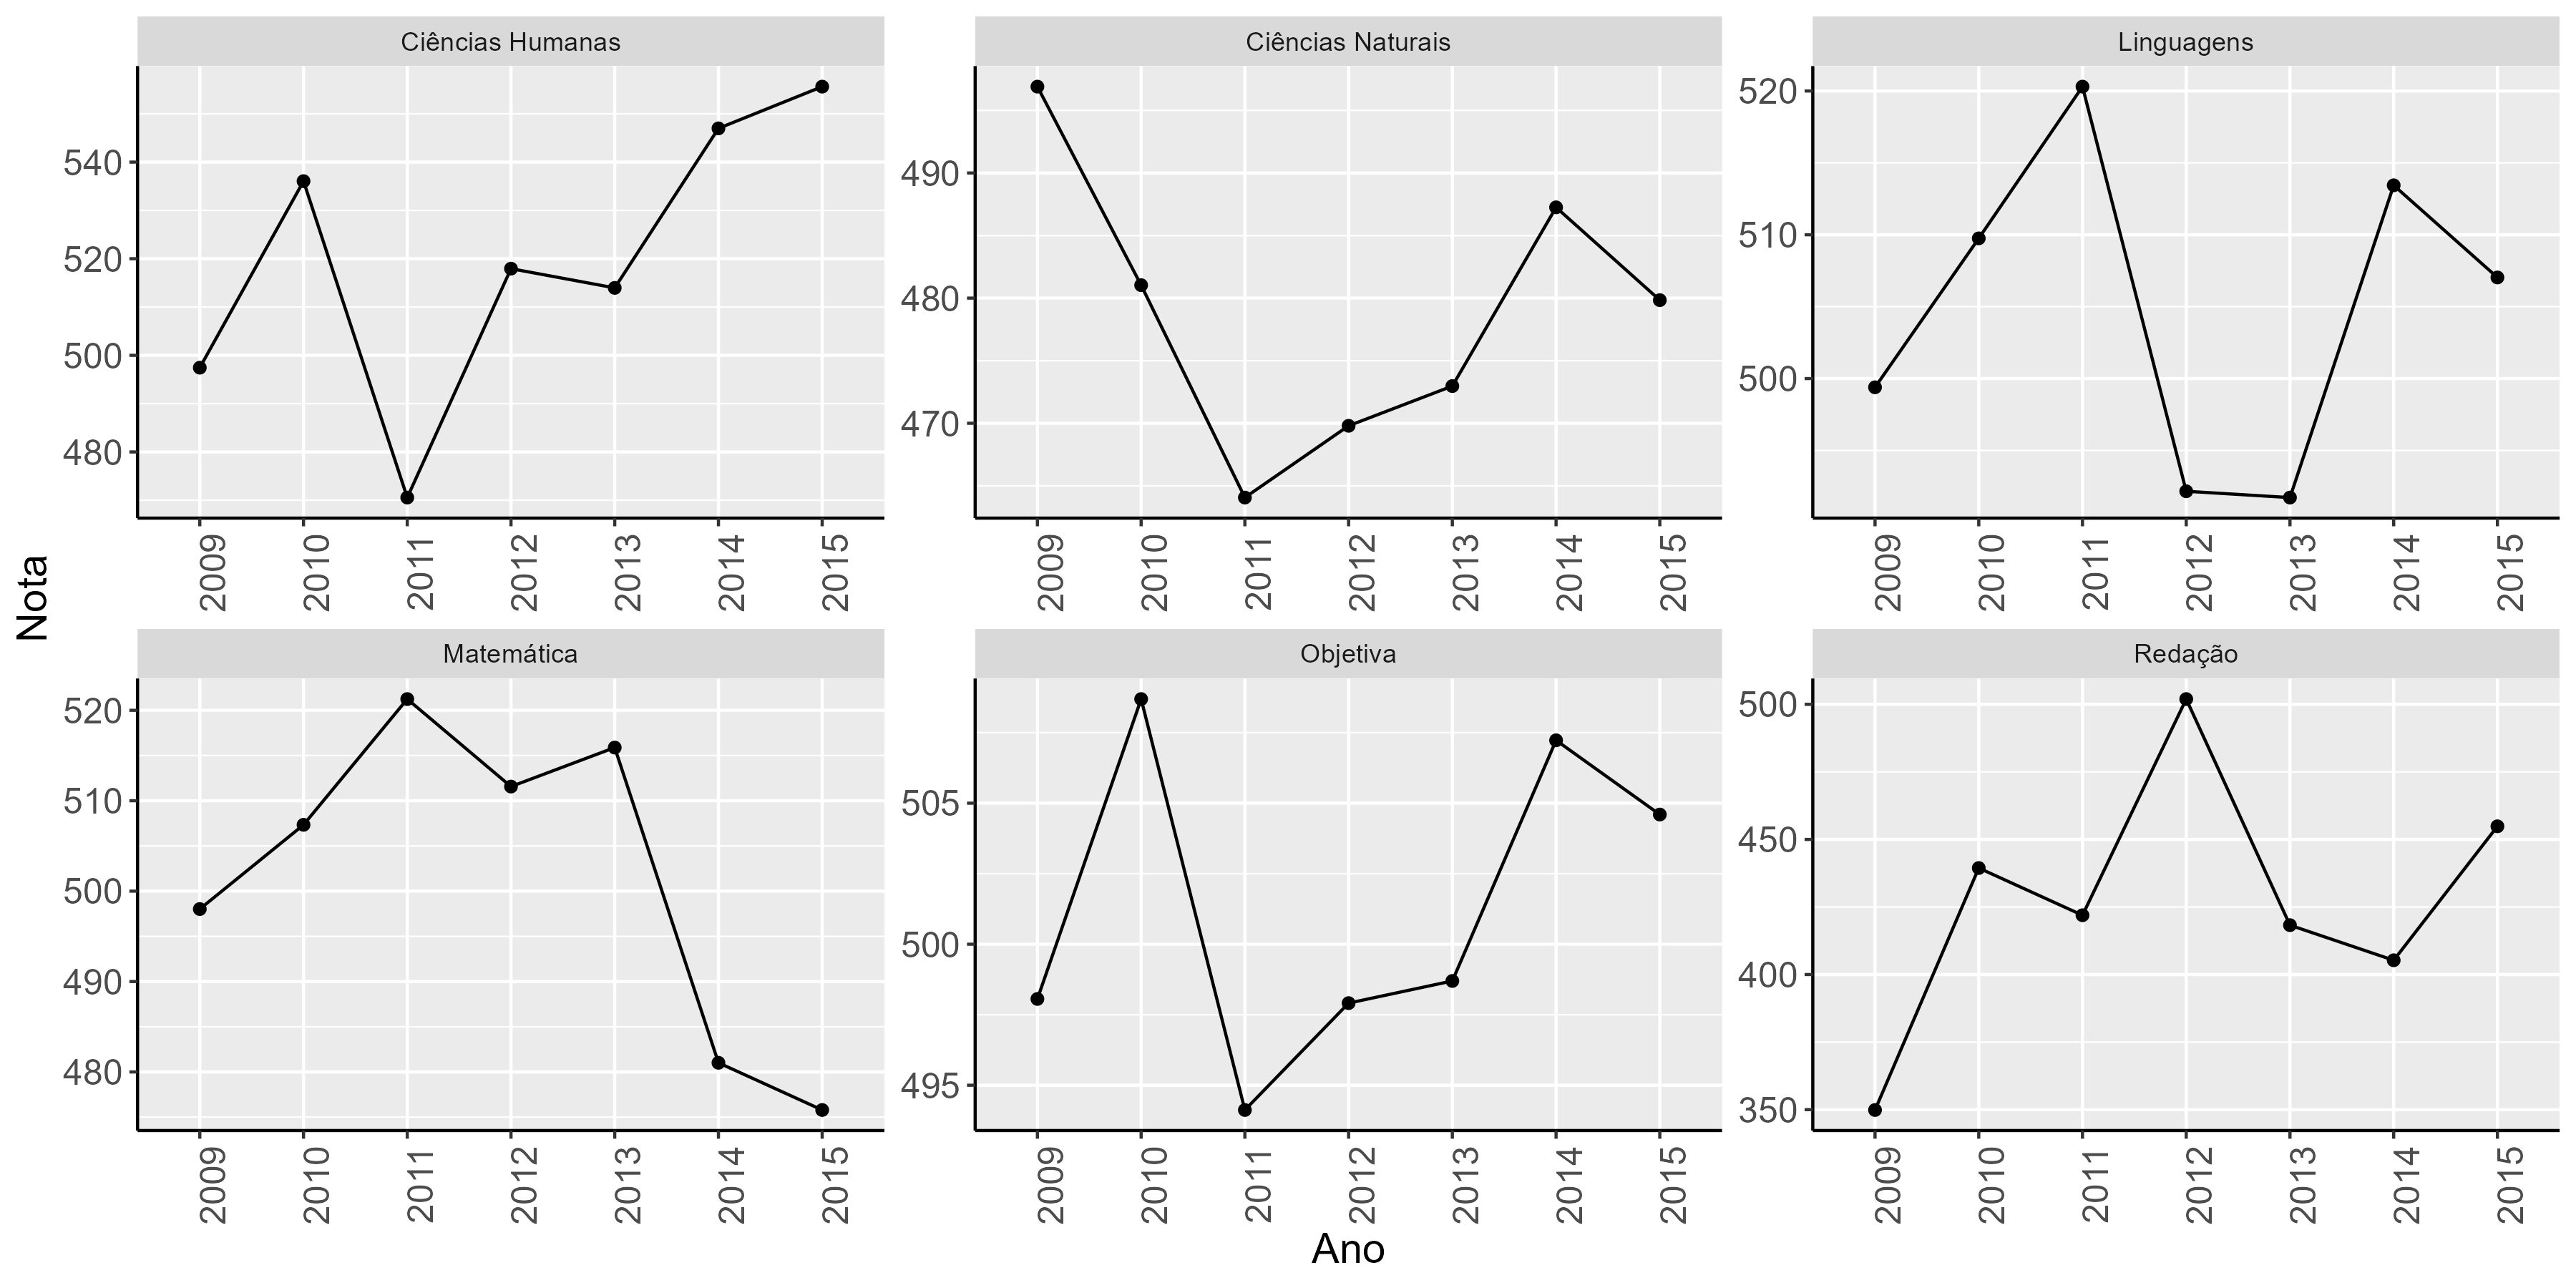
\includegraphics[width=0.95\textwidth]{Charts/serie_media_notas.png}
    \legend{Fonte: Elaboração própria com dados do INEP.}  
    \label{fig:serie_medi_notas}
\end{figure}

De acordo com a Pesquisa Nacional por Amostra de Domicílios Contínua (PNAD), em 2022, apenas um pouco mais da metade da população brasileira completou o ensino básico, enquanto 18\% dos jovens de 14 a 29 anos (cerca de 52 milhões de pessoas) não concluíram o ensino médio, seja por falta de frequência ou abandono. 

\begin{figure}[H]
    \centering
    \caption{Evolução dos indicadores educacionais}
    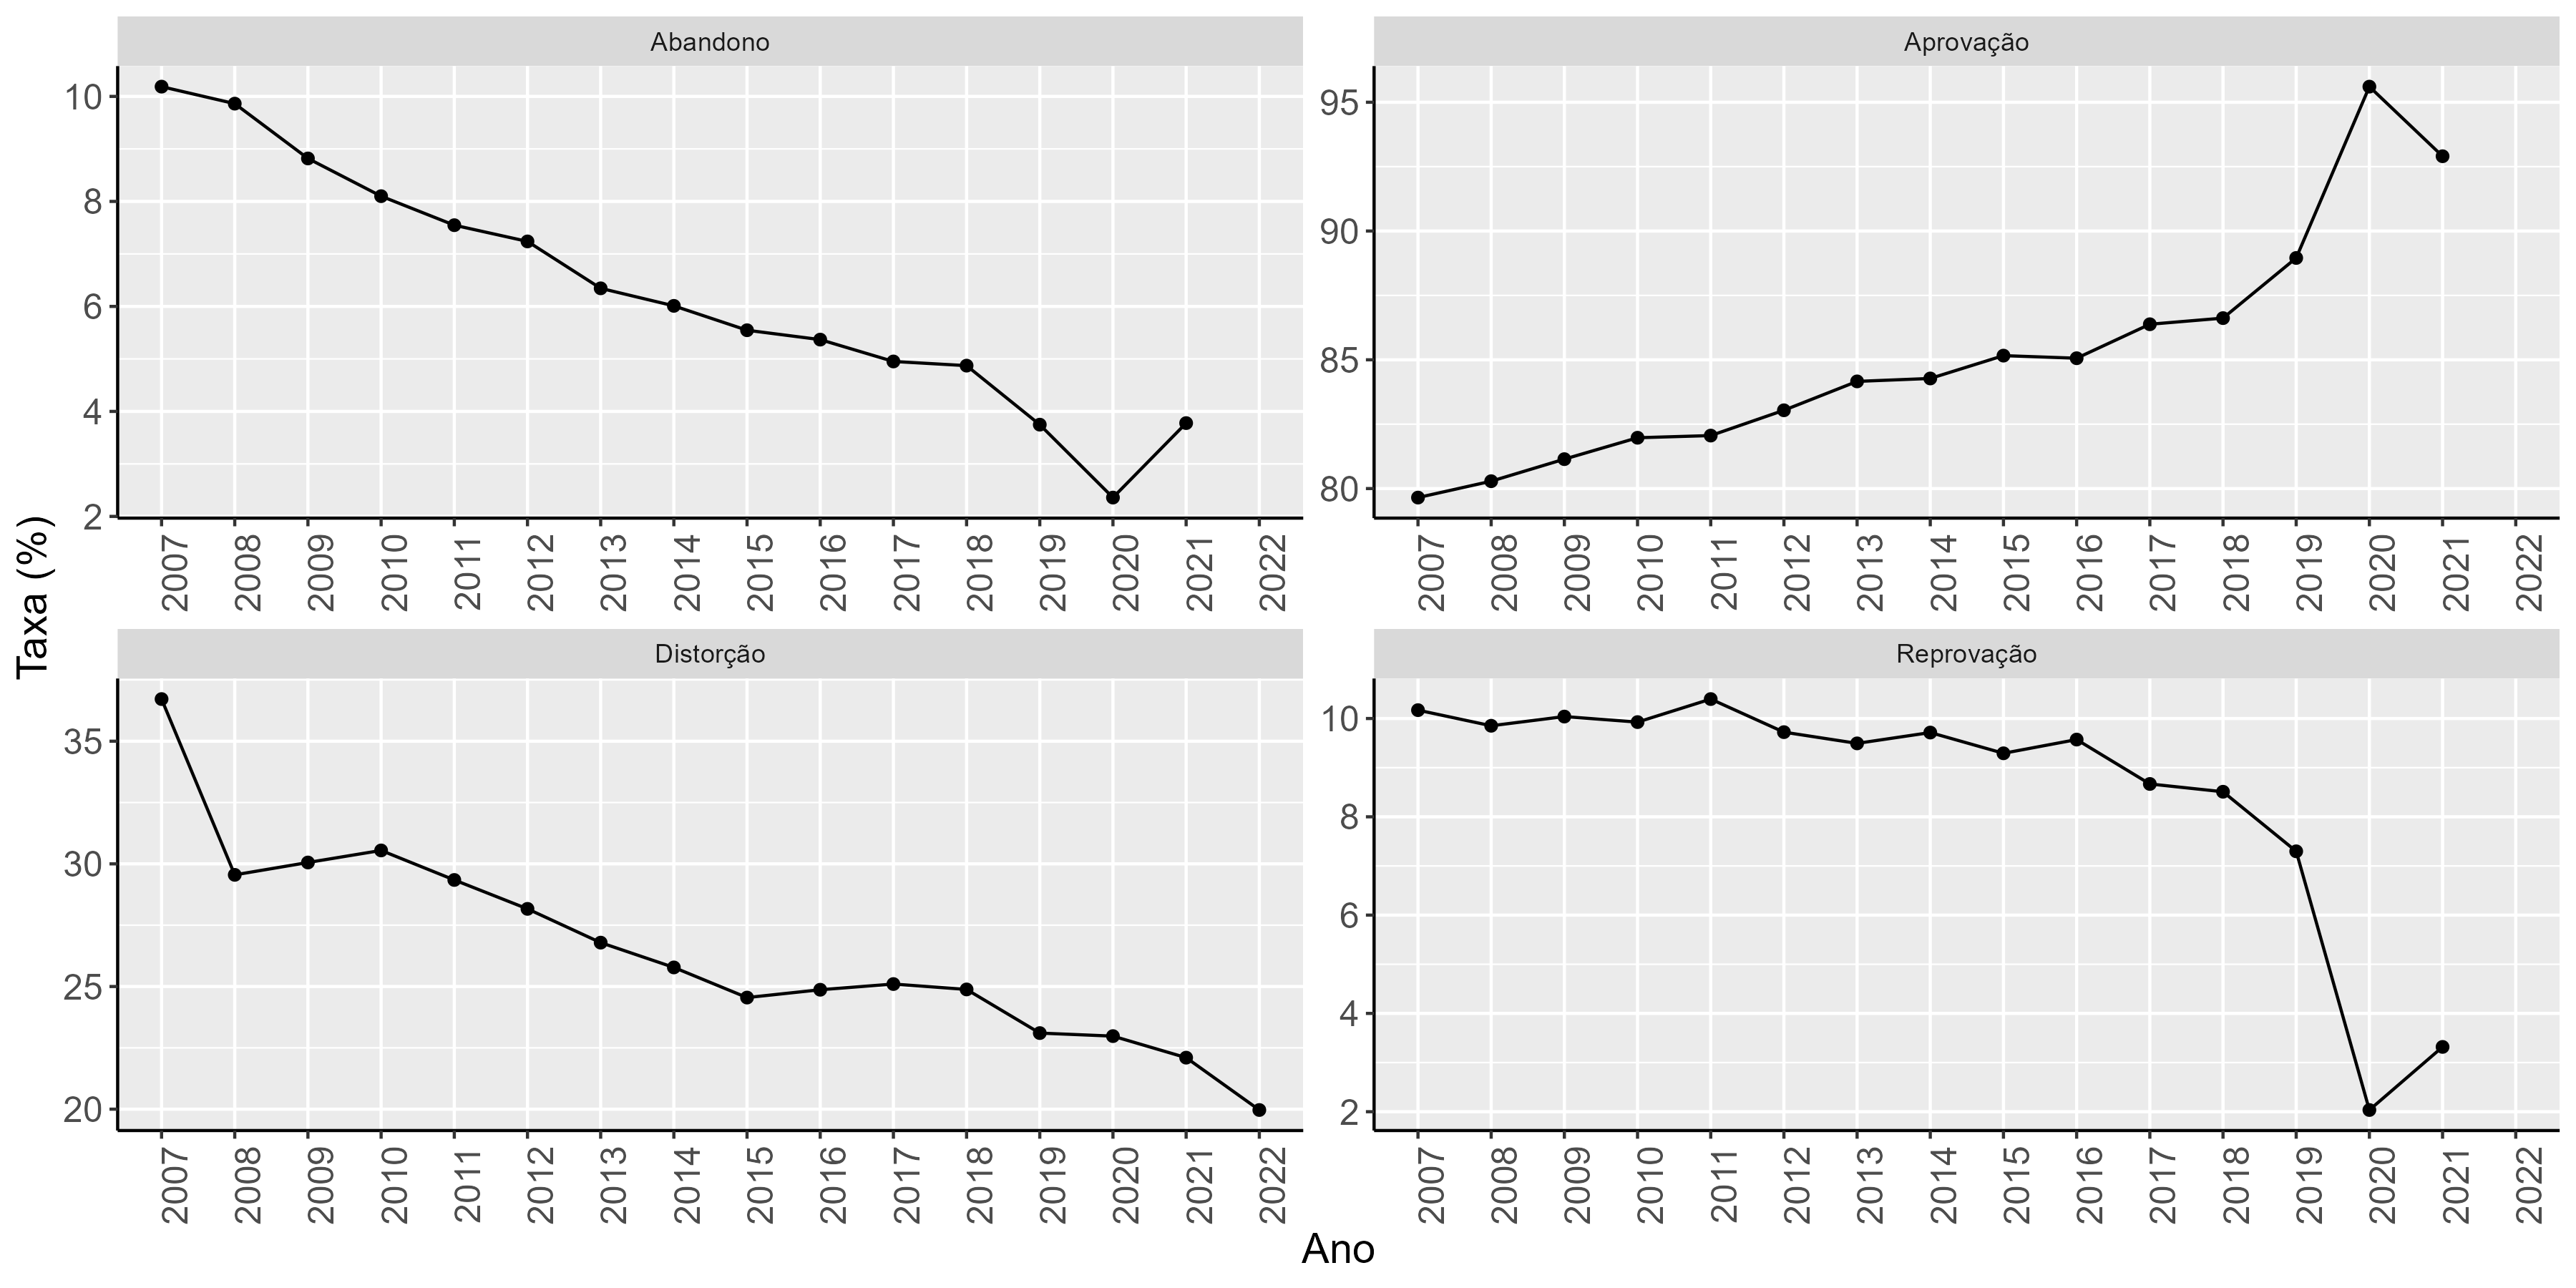
\includegraphics[width=0.95\textwidth]{Charts/serie_media_indicadores.png}
    \legend{Fonte: Elaboração própria com dados do INEP.}  
    \label{fig:serie_medi_indicadores}
\end{figure}

Diante desse cenário, os formuladores de políticas públicas buscam aprimorar continuamente a qualidade da educação. Sendo uma das medidas adotadas a expansão da jornada escolar, alcançada por meio de programas que aumentam a carga horária diária ou o número de dias letivos. Esses programas incluem atividades extracurriculares, reforço escolar, alimentação e orientação de vida, com o objetivo de transformar a escola em um agente integral na formação dos alunos como cidadãos.

No Brasil, essa abordagem é respaldada pelo Plano Nacional de Educação e foi implementado a partir de 2008, começando com o programa "Mais Educação". Este programa do governo federal visava estender a jornada escolar para pelo menos 7 horas diárias, em comparação às 4 horas de uma escola comum.

Para o ensino médio, o programa federal "Ensino Médio Integral" (EMI) foi lançado em 2004 como uma parceria público-privada. O EMI tem como objetivo formar os alunos em aspectos cognitivos, profissionais, pessoais e sociais, além de adotar critérios de gestão que incluem incentivos e critérios de contratação.

Neste trabalho, buscamos compreender se o programa EMI está cumprindo seu propósito de melhorar a qualidade da educação brasileira. Utilizaremos o método de \textit{staggered difference in differences} por \cite{CB_2021}, uma abordagem inédita para avaliar o programa ao nível desejado.

É relevante observar que vários estudos anteriores exploraram o potencial impacto de programas de ensino integral no Brasil, apresentando resultados mistos, como evidenciado por \cite{Oliveira_2008}, \cite{Almeida_2016}, \cite{Pereira_2011}, \cite{Filho_2012}, \cite{Xerxenevsky_2012}, \cite{Oliveira_2018} \cite{Kawahara_2019}. Analisaremos esses resultados de forma mais detalhada no capítulo subsequente.

A estrutura deste trabalho é a seguinte: na seção \ref{revisao}, analisaremos a literatura sobre os efeitos do ensino em tempo integral, tanto no Brasil quanto no cenário global. Na seção \ref{programa}, exploraremos as características, o funcionamento e os objetivos do programa EMI. A seção \ref{dados} apresentará as fontes para os dados que serão utilizados no trabalho. Finalmente, a seção \ref{ecomometria} descreverá o método causal aplicado e na seção \ref{resultados} apresentaremos os resultados obtidos, bem como a comparação deles com a literatura.

Assim, este trabalho visa contribuir para o crescente corpo de literatura sobre os efeitos de programas de ensino em tempo integral em todo o mundo, oferecendo insights que podem auxiliar na avaliação, formulação e implementação de políticas públicas educacionais.

% --------------------------- Desenvolvimento ------------------------ %
\chapter{Revisão de Literatura} \label{revisao}

O tema da ampliação da jornada escolar tem sido objeto de investigação por diversos autores em contextos globais. A seguir, apresentamos uma variedade de estudos que oferecem insights valiosos sobre essa temática diversificada, abordando uma ampla gama de resultados, metodologias e amostras. A heterogeneidade de resultados pode ser atribuída, em grande parte, à multiplicidade de abordagens e características dos programas analisados.

\section{Resultado Teórico} \label{teoria}

Baseando-nos no modelo proposto por \cite{Levin_1987}, supomos que o aluno realiza duas atividades de produção: a atividade escolar \(Q_1\) e outra atividade \(Q_2\). As funções de quantidade são expressas como funções positivas na seguinte forma funcional:

\begin{equation}
\begin{aligned}
& Q_1 = f(C, S) \cdot e_1^{\alpha_1} + t_1^{\beta_1} \\
& Q_2 = k(X) \cdot e_2^{\alpha_2} + t_2^{\beta_2} \\
\end{aligned}
\end{equation}

Aqui, \(e_i\) representa o esforço alocado para a atividade, \(t_i\) o tempo dedicado a ela, \(p_i\) são os preços de cada atividade, \(\alpha_i\) e \(\beta_i\) são parâmetros tecnológicos associados a cada atividade, assumidos como positivos. Além disso, \(C\) representa o nível de capacidade do aluno, \(S\) o nível de recursos de aprendizagem disponíveis e \(X\) são outros fatores externos à escola.

Portanto, o estudante resolverá o seguinte problema de otimização:

\begin{equation}
\begin{aligned}
\max \quad & U = p_1 \cdot F(Q_1) + p_2 \cdot G(Q_2) \\
\textrm{s.a.} \quad & t_1 + t_2 \leq T\\
& e_1 \cdot t_1 + e_2 \cdot t_2 \leq E
\end{aligned}
\end{equation}

Ao maximizar, obtém-se o seguinte resultado de equilíbrio:

\begin{equation}
    \frac{p_1 \cdot (\partial F/ \partial Q_1)Q_1^*}{p_2 \cdot (\partial G/ \partial Q_2)Q_2^*} = \frac{k(X) \alpha_2}{f(C,S)\alpha_1} \cdot \frac{e_1^{*1-\alpha_1}t_1^{*1-\beta_1}}{e_2^{*1-\alpha_2}t_2^{*1-\beta_2}}
\end{equation}

Ao analisar o equilíbrio do modelo proposto, conclui-se que não existem cenários em que haja ganhos significativos na produção do aluno caso haja somente aumento no tempo dedicado à atividade. Isso decorre da observação de reduções no esforço quando o tempo de estudo é aumentado, resultando em resultados nulos ou até mesmo negativos.

No entanto, sob as características do programa, o equilíbrio pode ser interpretado de forma mais abrangente. Como detalhado no capítulo \ref{programa}, o EMI não apenas aumenta a carga horária, mas também introduz dispositivos que renovam o ambiente escolar, como recursos de aprendizagem e aprimoramento da gestão. Portanto, em termos do modelo teórico, podemos interpretar o programa como uma mudança nos coeficientes de produtividade da função de produção (\(\alpha_i\), \(\beta_i\)).

Consequentemente, podemos concluir que o programa resulta em um aumento na produtividade dos alunos, permitindo que eles aloquem mais tempo e esforço na atividade escolar conforme a produtividade de aprendizagem aumenta em relação à produtividade de outras atividades, conforme indicado pelos autores.

Com base nas conclusões teóricas estabelecidas, buscaremos testar se a implementação do programa EMI tem um impacto positivo nos resultados educacionais das escolas brasileiras, conforme desenvolvido no texto acima.
 
\section{Evidências ao redor do mundo}

Em um contexto latino americano, \cite{Bellei_2009} busca compreender como os estudantes chilenos de ensino médio foram afetados pelo programa de extensão da jornada escolar. Utilizando a metodologia de diferenças em diferenças, o autor encontra efeitos positivos em testes de matemática e português.

Segundo \cite{Meroni_2016}, a extensão da jornada escolar pode influenciar positivamente o desempenho acadêmico, parte de um processo cumulativo. Os autores propuseram uma análise abrangente dessas dinâmicas, examinando estudantes italianos de ensino médio no período de 2007 a 2010. Utilizando dados do Ministério de Educação, aplicaram o método de diferenças em diferenças com base na segunda fase do programa Quality and Merit Project (PQM). Os resultados da pesquisa indicam que, para os estudantes do sexo masculino, uma maior exposição à matemática está associada a um aumento na aversão a essa disciplina e a uma maior ansiedade diante de avaliações de linguagem. Por outro lado, para as estudantes do sexo feminino, a exposição à matemática parece contribuir para a redução da aversão a essa matéria e para um melhor desempenho em disciplinas de linguagem.

\section{Evidências para o Brasil}

No contexto brasileiro, encontramos uma série de estudos que examinam os efeitos da carga horária escolar no desempenho dos alunos. Um estudo notável conduzido por \cite{Filho_2012} utilizou dados do Sistema de Avaliação da Educação Básica (SAEB) de 2003 para investigar os determinantes do desempenho de alunos de escolas públicas no Brasil. Este estudo revelou que alunos que frequentavam a escola por mais de 4 horas diárias apresentavam maior proficiência em matemática em comparação àqueles com menos de 4 horas de aulas diárias.

Outra pesquisa relevante, realizada por \cite{Oliveira_2008}, utilizou dados do SAEB referentes a 2005, com foco nos alunos da 4ª série do ensino fundamental. Neste estudo, foram aplicadas técnicas de \textit{matching} para investigar se a redução do tamanho das turmas e o aumento da carga horária escolar influenciaram o rendimento dos alunos. Os resultados apontaram uma estimativa de tratamento médio de 8,36 pontos na proficiência em matemática para os alunos que experimentaram um acréscimo de uma hora na jornada diária, indicando uma relação positiva entre a carga horária e o desempenho acadêmico.

Por outro lado, uma pesquisa conduzida por \cite{Aquino_2011} buscou analisar os efeitos do programa Escola de Tempo Integral. Utilizando dados do Sistema de Avaliação de Rendimento Escolar do Estado de São Paulo (SARESP) dos anos de 2007 e 2008, esta investigação focalizou os alunos da 8ª série do ensino fundamental. Por meio de métodos de \textit{matching} e o método de diferenças em diferenças, a autora não encontrou evidências de efeitos significativos no rendimento em matemática, mas observou efeitos positivos no rendimento em português.

No Brasil, um programa amplamente avaliado é o programa federal Mais Educação. \cite{Pereira_2011} utilizou dados disponibilizados pela secretaria do programa para compreender seus impactos sobre a taxa de abandono escolar, aprovação e rendimento escolar de alunos em todo o país e, especificamente, no estado de Minas Gerais. Por meio do método de diferenças em diferenças, o autor concluiu que o programa não teve efeitos significativos sobre a taxa de aprovação, mas exerceu um efeito positivo na redução da taxa de abandono escolar. Quanto ao rendimento, concluiu que o programa não produziu efeitos significativos sobre os alunos de Minas Gerais.

Utilizando dados da Prova Brasil para os anos de 2007 e 2009 no estado do Rio Grande do Sul, \cite{Xerxenevsky_2012} empregou métodos de propensity score matching e diferenças em diferenças para avaliar o impacto do programa Mais Educação. O autor descobriu que o programa teve impacto positivo no desempenho escolar em língua portuguesa para alunos da 4ª série, mas impacto negativo no desempenho em matemática. Para alunos da 8ª série, não foram observados efeitos significativos para testes de língua portuguesa e matemática.

\cite{Almeida_2016} e \cite{Gandra_2017} utilizaram dados do Censo Escolar em diferentes períodos e aplicaram métodos como propensity score matching e regressão de diferenças em diferenças para avaliar o impacto do programa. Enquanto \cite{Almeida_2016} observou impactos negativos no rendimento em matemática, mas ausência de impacto nas taxas de abandono e aprovação, \cite{Gandra_2017} encontrou impactos negativos no rendimento em matemática e português para as turmas do 5º ano, com maior magnitude nas escolas que aderiram ao programa por mais tempo.

\cite{Oliveira_2018} também utilizou dados do Censo Escolar, aplicando métodos de propensity score matching e regressão com descontinuidade, mas não encontrou melhorias nas taxas de abandono, aprovação, reprovação, proficiências e no Índice de Desenvolvimento da Educação Básica (IDEB).

Há também estudos que buscam compreender outro programa presente no Brasil, o Ensino Médio Integral (EMI), o qual é objeto de estudo do presente texto. Ao estudarem a mesma intervenção utilizando métodos diferentes, \cite{Kawahara_2019} e \cite{Rosa_2022a} chegam a conclusões semelhantes sobre os efeitos do programa nas notas em testes padronizados. O primeiro procura compreender como o programa impacta o rendimento dos alunos de escolas públicas. Utilizando o método de diferenças em diferenças dinâmico, o autor constatou que há efeitos positivos e crescentes no tempo sobre os testes padronizados de matemática e português. O autor também indica a possibilidade de que o programa também traga efeitos indiretos. Esses efeitos podem incluir mudanças resultantes da mobilidade de alunos entre escolas, alterações na estrutura escolar e no ambiente socioeconômico dos alunos, bem como efeitos relacionados à autoseleção de alunos e professores. Já o segundo estuda o mesmo programa, com foco nas escolas de Pernambuco, estado onde o programa se iniciou. Para o contexto deste trabalho, os resultados obtidos por meio do método de \textit{staggered difference in differences} proposto por \cite{CB_2021} mostram que ao longo dos anos após a implementação da política, há um efeito positivo e crescente sobre os resultados dos alunos em testes padronizados, de modo que características observáveis dos alunos possivelmente não alteram os resultados encontrados. 

\section{Evidências de médio e longo prazo}

Outros estudos buscam compreender efeitos além da sala de aula. Para isso, os estudos buscam entender efeitos de médio e longo prazo dos estudantes expostos a programas de ensino integral. Como objeto de estudo, os artigos relacionam o programa com resultados econômicos.

Conforme evidenciado por \cite{Barros_2022}, o ensino médio em tempo integral pode acarretar efeitos positivos a médio e longo prazo tanto para os alunos quanto para a sociedade em geral. Com base nos resultados apresentados pelos autores, espera-se que esses efeitos se manifestem de forma positiva em indicadores como empregabilidade, renda, produtividade e crescimento econômico.

As evidências mostradas por \cite{Dominguez_2020} nos permite observar que ao ser exposto ao programa de ensino médio integral há aumento das chances dos alunos de concluir o ensino básico e superior, sendo este um resultado positivo do programa. Caso a exposição ao ensino médio integral traga efeitos de proficiência, como mostrado por \cite{Barros_2019}, podemos esperar que o aluno possa ter uma elevação em seu rendimento, como evidenciado por \cite{Barros_2021}.
\chapter{O Programa Ensino Médio Integral} \label{programa}
No início dos anos 2000, o Ginásio Pernambucano, o colégio mais antigo do Brasil, passou por uma reforma promovida pela sociedade civil. Uma das mudanças significativas incluiu a transição para o modelo de ensino integral. Desde então, esse programa foi adotado pelo governo federal e expandido para todos os estados do Brasil, com aproximadamente 544 escolas participantes em 2015 \cite{Kawahara_2019}. A expansão do programa é realizada com o apoio de um instituto voltado à políticas educacionais, o Instituto de Corresponsabilidade pela Educação (ICE).

O principal objetivo desse programa é atender à Meta 6 do Plano Nacional de Educação (PNE), que busca expandir o ensino em tempo integral. Para alcançar essa meta, o programa adota uma abordagem pedagógica baseada no conceito de "Projeto de Vida". Isso significa que as escolas não apenas se concentram no desenvolvimento cognitivo dos alunos, mas também no seu desenvolvimento socioemocional. Os estudantes são incentivados a se tornarem protagonistas de suas próprias vidas, tomando decisões responsáveis, enquanto recebem o apoio de profissionais envolvidos ativamente em suas jornadas educacionais.

Além da abordagem pedagógica, o programa também reorganiza a gestão das escolas participantes. Isso envolve critérios específicos para a contratação de professores e gestores, sistemas de incentivos para os educadores e métricas de gestão para avaliar o progresso.

A transição de uma jornada escolar de 4 horas diárias para 9 horas requer modificações na infraestrutura das escolas. Nesse sentido, o instituto colabora com as secretarias de educação na seleção das escolas e, nas fases iniciais do programa, oferece apoio financeiro para a compra de materiais escolares, construção de novas instalações e pagamento de bônus de desempenho e alimentação. Durante essa fase inicial, o instituto também supervisiona de perto a implementação do programa. Uma vez que o programa é estabelecido, as escolas têm mais autonomia para gerenciá-lo, bem como para administrar suas instalações e sistemas, uma vez que o instituto retira sua supervisão direta.

Até o ano de 2022, 6400 das 19870 escolas no Brasil apresentavam o ensino médio integral, estando concentradas nas regiões Sudeste e Nordeste do país, como apresentado na Figura \ref{fig:brazil_schools}. 

\begin{figure}[H]
    \centering
    \caption{Quantidade de escolas com ensino integral no ano de 2022}
    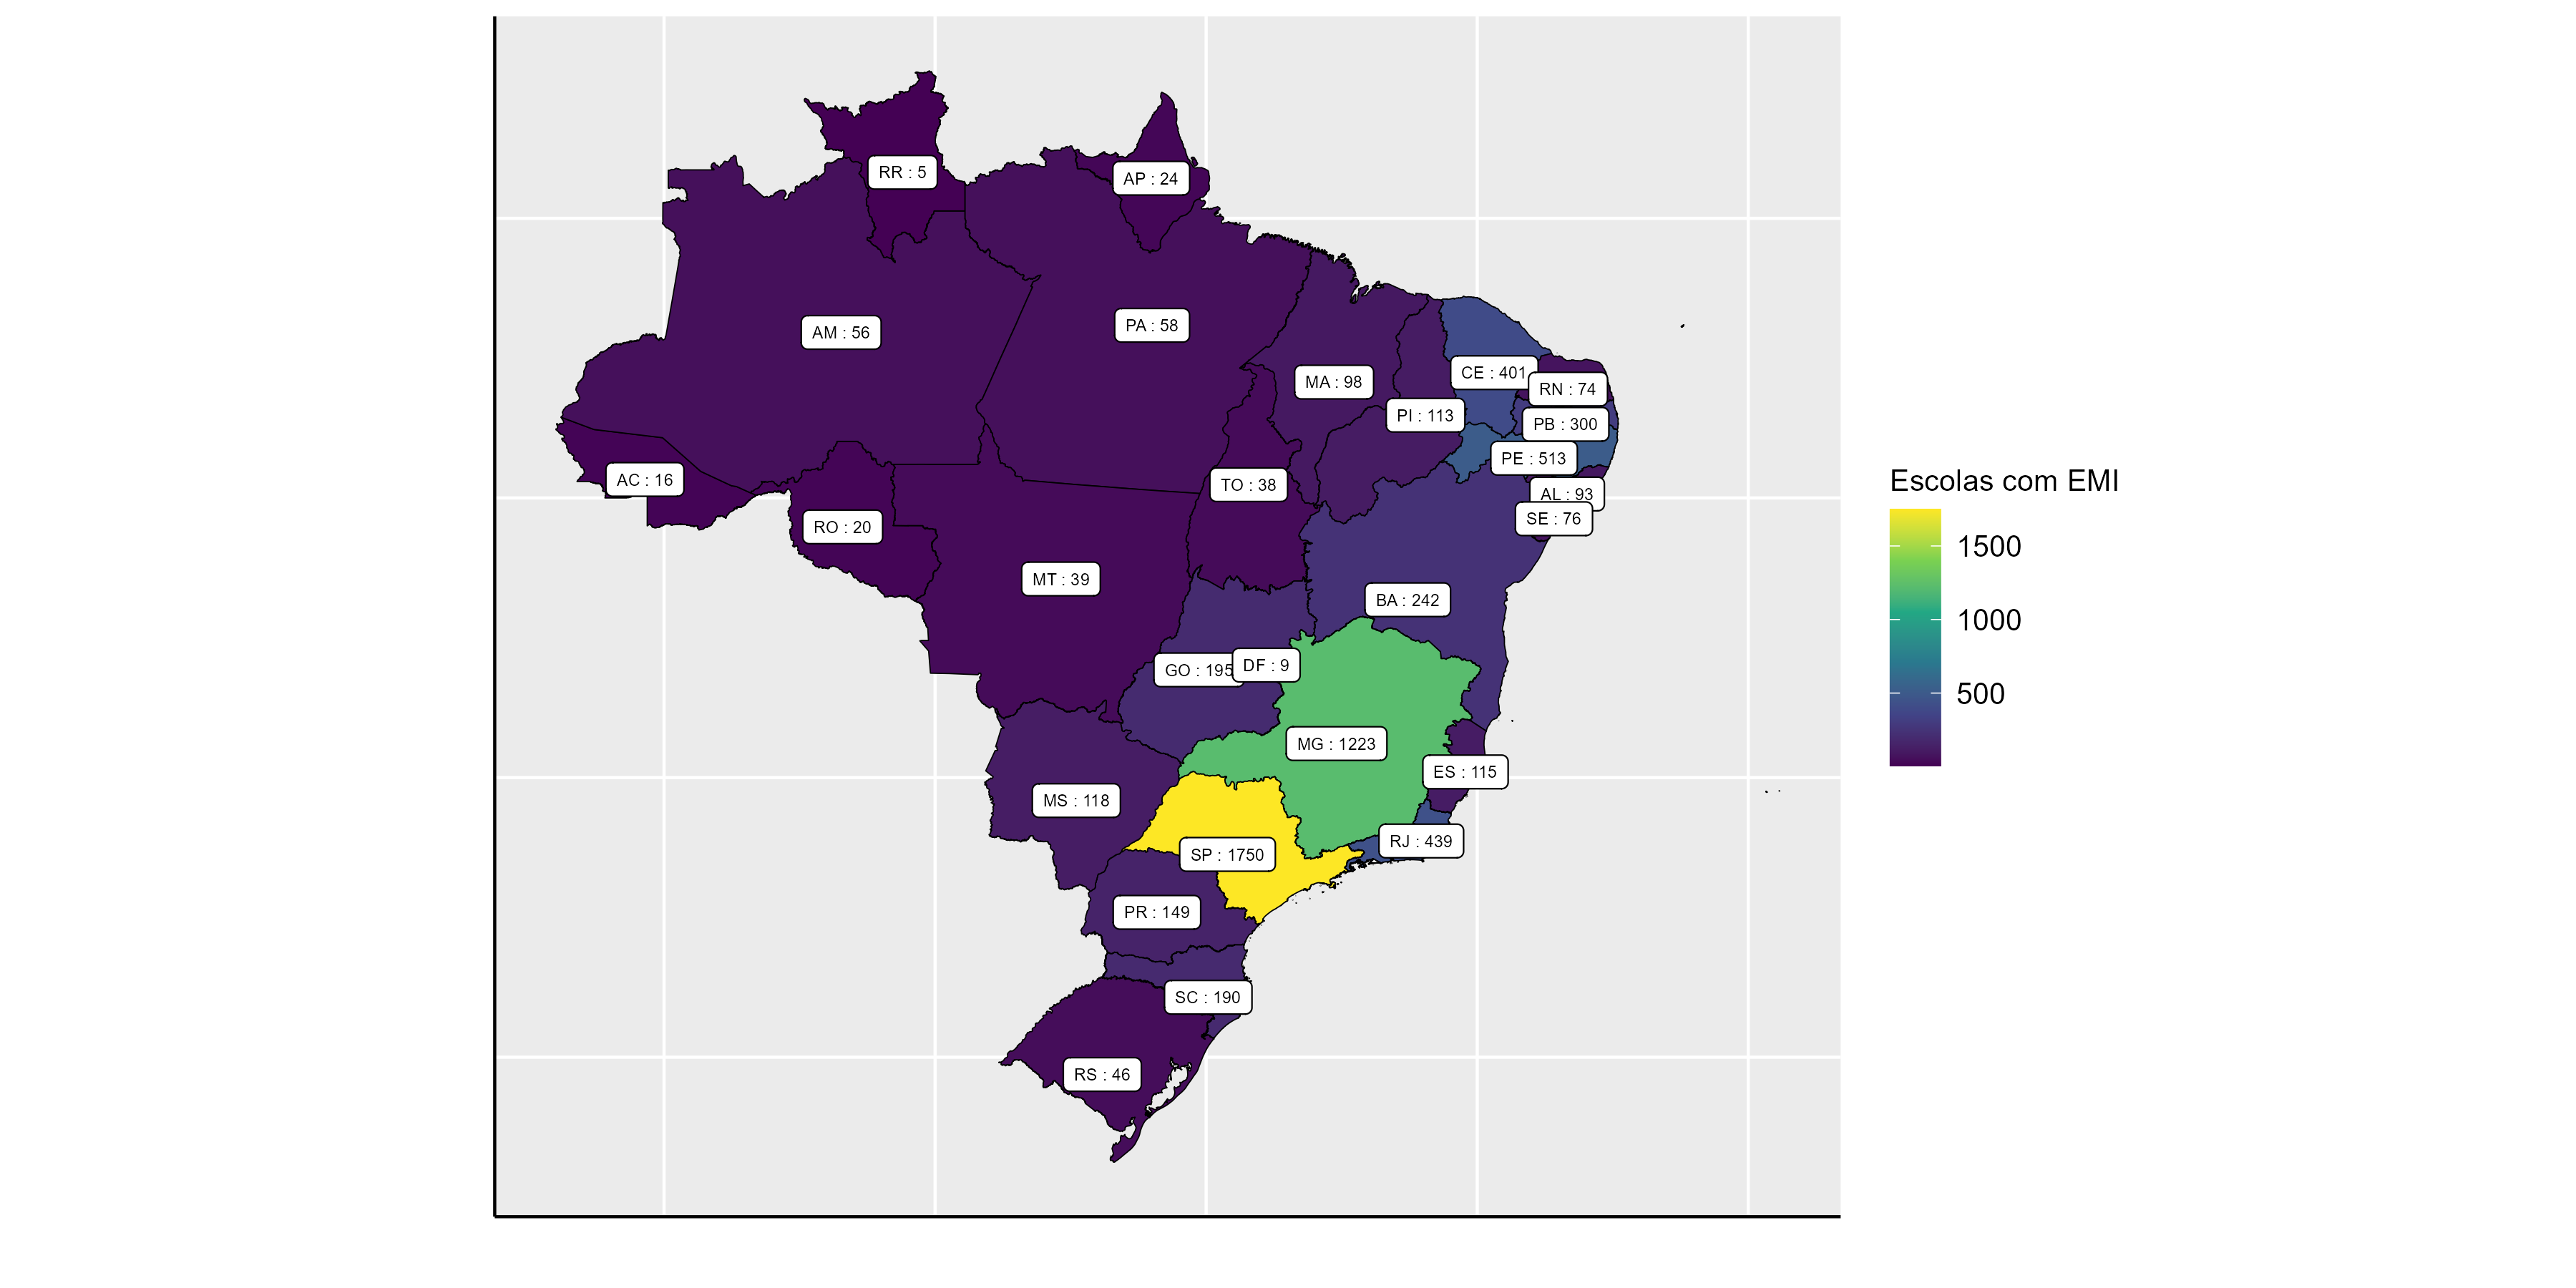
\includegraphics[width=1.15\textwidth]{Charts/brazil_schools.png}
    \legend{Fonte: Elaboração própria com dados do Instituto Sonho Grande, 2024.}  
    \label{fig:brazil_schools}
\end{figure}

\begin{figure}[H]
  \centering
  \caption{Percentual de escolas integrais no ensino médio}
  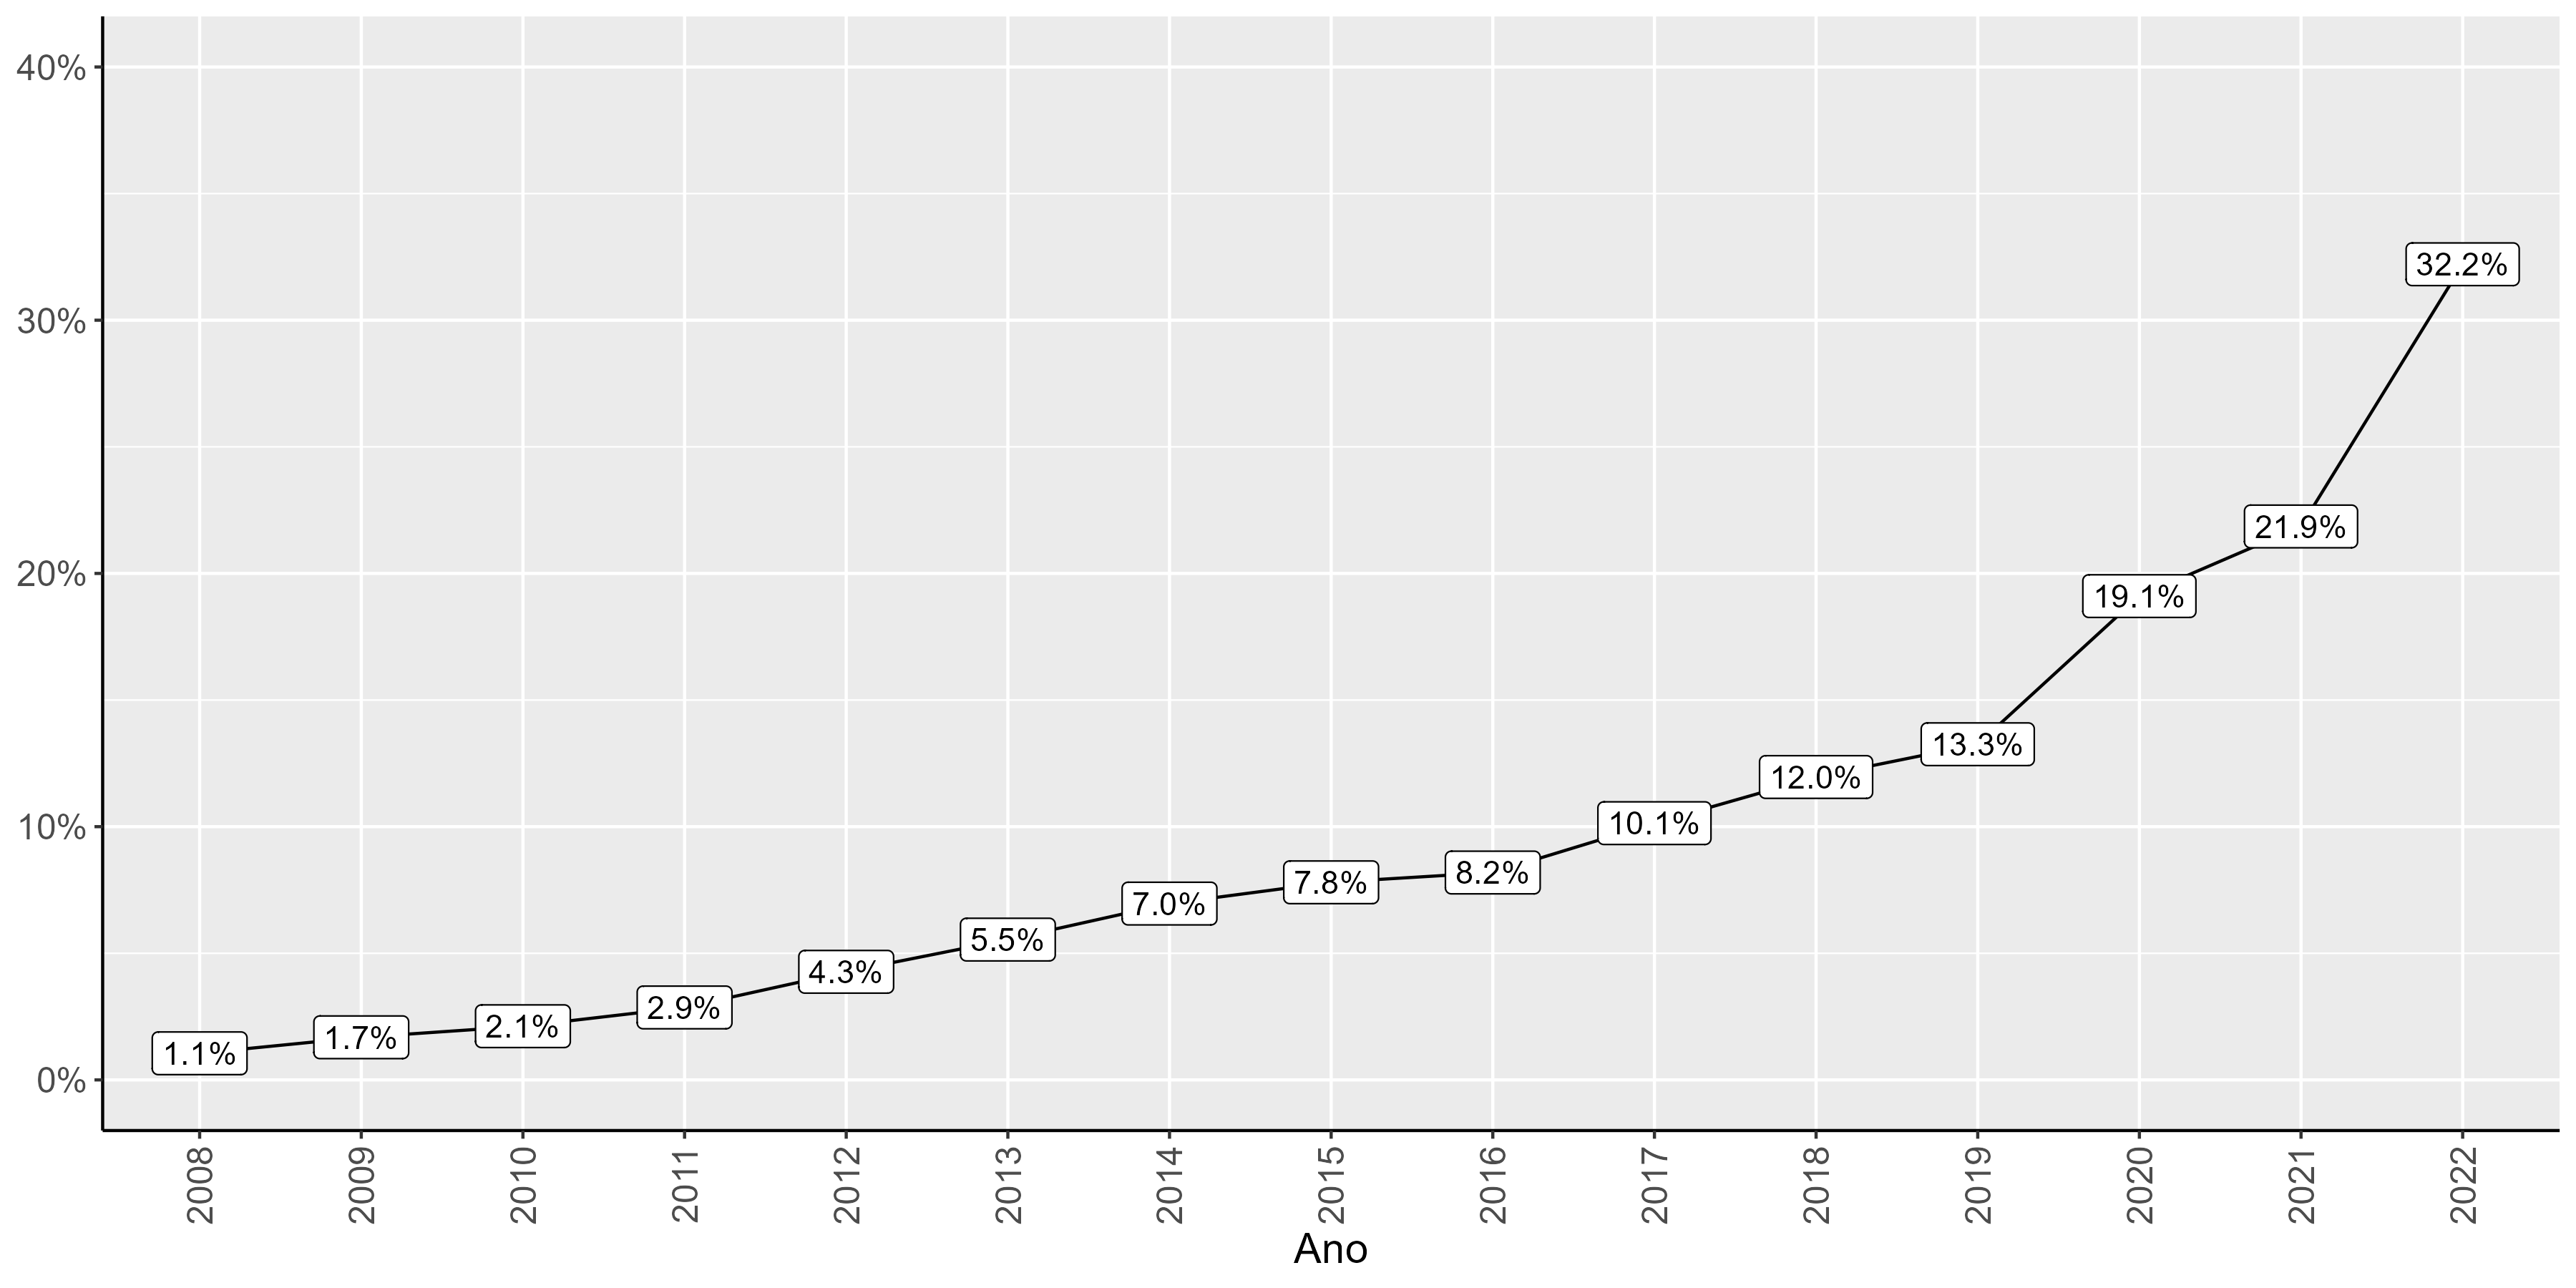
\includegraphics[width=1\textwidth]{Charts/serie_escolas_integral.png}
  \legend{Fonte: Elaboração própria com dados do Instituto Sonho Grande, 2024.}  
  \label{fig:serie_escolas_integral}
\end{figure}
\chapter{Base de Dados} \label{dados}

Os dados utilizados neste trabalho são divididos em dois conjuntos, tendo como fontes o Instituto Nacional de Estudos e Pesquisas Educacionais Anísio Teixeira (INEP), o Instituto Corresponsabilidade pela Educação (ICE) e o Instituto Sonho Grande (ISG).

O Censo Escolar, realizado anualmente pelo INEP, fornece informações detalhadas sobre as estruturas físicas e organizacionais das escolas públicas e privadas do ensino básico no Brasil. Este conjunto de dados oferece um panorama escolar, especialmente para instituições de ensino médio.

Além disso, o Exame Nacional do Ensino Médio (ENEM), também organizado pelo INEP anualmente, é um exame voluntário que avalia o nível de aprendizado dos alunos das escolas públicas e privadas do ensino médio do Brasil em cinco áreas de competência (linguagens, matemática, ciências naturais, ciências humanas e redação). Os resultados do ENEM são frequentemente usados pelos estudantes em suas candidaturas para ingresso no ensino superior, tanto em universidades federais quanto em diversas instituições privadas. Além de avaliar o desempenho dos alunos nessas áreas, o exame inclui um questionário socioeconômico.

Os dados administrativos do ICE apresentam informações sobre as escolas que aderiram ao programa, indicando o ano de ingresso e detalhes dos elementos implementados em cada instituição. 

Os dados do ISG apresentam o ano em que a escola aderiu ao programa, bem como certas características sobre ela.

O primeiro conjunto foi fornecido por \cite{Kawahara_2019}. Ele provêm do INEP e de informações administrativas do ICE. Este conjunto diz respeito aos resultados das escolas nas provas do ENEM  durante os anos de 2009 e 2015, abrangendo escolas de ensino médio situadas nos estados de São Paulo, Rio de Janeiro, Espírito Santo, Ceará, Pernambuco e Goiás. 

Já o segundo conjunto de dados foi construído com base nas informações das escolas que participam do programa, disponibilizadas pelo ISG. Este conjunto diz respeito a indicadores educacionais do INEP (taxa de aprovação, reprovação, abandono e distorção) entre os anos de 2007 e 2022 para escolas localizadas em todo território brasileiro \footnote[1]{\textit{Uma descrição das variáveis presentes em ambos conjuntos está disponível no Apêndice \ref{apendice_descricao}.}}.

Na Tabela \ref{tab:descritiva_resultados} conseguimos ver estatísticas descritivas para as variáveis de resultados acadêmicos, enquanto nas Tabelas \ref{tab:desc_ice} e \ref{tab:desc_censo} é possível observer estatísticas descritivas para as variáveis de caracterísitcas das escolas nos dois conjuntos de dados utilizados. Com base na Tabela \ref{tab:descritiva_resultados} podemos observar o baixo desempenho dos alunos do ensino médio brasileiro no ENEM, sendo seu rendimento médio aquém do nível máximo do teste. No mais, observarmos médias mais baixas em diversos indicadores educacionais entre as escolas tratadas, havendo significância estatística que sustente esta diferença.

\begin{table}[H]
\centering
\caption{Estatísticas descritivas para variáveis de resultados escolares}
\label{tab:descritiva_resultados}
\begin{tabular}{lcccc}
\hline
                          &Média& Desvio Padrão & \multicolumn{2}{c}{Teste-T Para Médias}\\
\cline{4-5}
                          & & & Diferença & P-Valor \\
\hline
Nota em matemática        & 501,4 &74,4 &-32,7& <0,001\\
Nota em linguagens        & 504,8& 49,8&-22,1& <0,001\\
Nota em ciências naturais & 478,8&51,1 &-25,9& <0,001\\
Nota em ciências humanas  & 520,1& 520,1 &-26,2& <0,001\\
Nota em redação           & 427,1& 451,0&-15,1& <0,001\\
Nota geral em objetivas          & 501,4& 51,0&-26,2& <0,001\\
Taxa de abandono          & 6,2&8,7&7,3& <0,001\\
Taxa de reprovação        & 8,5&8,8&5,1& <0,001\\
Taxa de distorção         & 26,3&20,6&21,9& <0,001\\
Taxa de aprovação         & 85,3&13,3&-12,3& <0,001\\ 
\hline
\end{tabular}
    \legend{Fonte: Elaboração própria, 2024.} 
\end{table}

\begin{table}[H]
  \centering
  \caption{Descritivas das características escolares no primeiro conjunto de dados}
  \label{tab:desc_ice}
  \begin{tabular}{lcc}
  & Média& Desvio Padrão \\
  \hline
  Mora com mais de 6 pessoas (\%) & 0.050 & 0.090 \\
  Renda familiar acima de 5 salários mínimos (\%) & 0.170 & 0.251 \\
  Já trabalhou ou procurou emprego (\%) & 0.439 & 0.303 \\
  Número de mulheres no EM 1 & 53.407 & 63.183 \\
  Número de mulheres no EM 2 & 45.012 & 52.181 \\
  Número de mulheres no EM 3 & 40.019 & 46.544 \\
  Zona rural (\%) & 0.038 & 0.192 \\
  Ativa (\%) & 1.000 & 0.000 \\
  Prédio (\%) & 0.990 & 0.101 \\
  Diretoria (\%) & 0.949 & 0.219 \\
  Biblioteca (\%) & 0.558 & 0.497 \\
  Sala de leitura (\%) & 0.478 & 0.500 \\
  Laboratório de informática (\%) & 0.872 & 0.334 \\
  Laboratório de ciências (\%) & 0.453 & 0.498 \\
  Quadra de esportes (\%) & 0.792 & 0.406 \\
  Internet (\%) & 0.967 & 0.178 \\
  Coleta de lixo (\%) & 0.988 & 0.108 \\
  Eletricidade (\%) & 0.999 & 0.030 \\
  Água potável (\%) & 0.958 & 0.201 \\
  Esgoto (\%) & 0.829 & 0.376 \\
  Mulheres no EM 1 (\%) & 0.501 & 0.089 \\
  Mulheres no EM 2 (\%) & 0.528 & 0.095 \\
  Mulheres no EM 3 (\%) & 0.545 & 0.103 \\
  Alunos brancos no EM 1 (\%) & 0.579 & 0.273 \\
  Alunos brancos no EM 2 (\%) & 0.588 & 0.279 \\
  Alunos brancos no EM 3 (\%) & 0.593 & 0.283 \\
  Alunos no EM 1 que utilizam transporte público (\%) & 0.179 & 0.301 \\
  Alunos no EM 2 que utilizam transporte público (\%) & 0.178 & 0.303 \\
  Alunos no EM 3 que utilizam transporte público (\%) & 0.175 & 0.301 \\\hline
  \end{tabular}
      \legend{Fonte: Elaboração própria, 2024.} 
  \end{table}
  
  \begin{table}[H]
    \centering
    \caption{Descritivas das características escolares no segundo conjunto de dados}
    \label{tab:desc_censo}
    \begin{tabular}{lcc}
    & Média& Desvio Padrão \\
    \hline
    Zona rural (\%) & 0.129 & 0.335 \\
    Ativa (\%) & 1.000 & 0.000 \\
    Prédio (\%) & 0.985 & 0.120 \\
    Diretoria (\%) & 0.919 & 0.273 \\
    Biblioteca (\%) & 0.668 & 0.471 \\
    Sala de leitura (\%) & 0.314 & 0.464 \\
    Laboratório de informática (\%) & 0.849 & 0.358 \\
    Laboratório de ciências (\%) & 0.427 & 0.495 \\
    Quadra de esportes (\%) & 0.542 & 0.498 \\
    Internet (\%) & 0.906 & 0.292 \\    
    Coleta de lixo (\%) & 0.924 & 0.266 \\
    Eletricidade (\%) & 0.993 & 0.085 \\
    Água potável (\%) & 0.880 & 0.324 \\
    Esgoto (\%) & 0.600 & 0.490 \\
    \hline
  \end{tabular}
    \legend{Fonte: Elaboração própria, 2024.} 
    \end{table}
\chapter{Estratégia Empírica} \label{ecomometria}

Nesta seção, descreveremos a metodologia que será empregada para avaliar o impacto do Programa Ensino Médio Integral (EMI) no contexto brasileiro. A abordagem metodológica é fundamental para garantir uma análise robusta e precisa dos efeitos do programa. Para isso, utilizaremos o método de \textit{staggered differences in differences} proposto por \cite{CB_2021}.

Como citado na revisão de literatura, diversos trabalhos ao redor do mundo já tentaram adotar estratégias de inferência causal para avaliar programas relacionados ao aumento da carga horária escolar. Para isso, tais estudos tendem a utilizar a metodologia de diferenças-em-diferenças, consolidada na comparação de grupos de tratamento e controle.

Uma das abordagens mais utilizadas é denominada \textit{two-way fixed effect differences in differences}. Em uma especificação estática, podemos escrever tal abordagem da seguinte forma:

\begin{equation}
    Y_{it} = \alpha_0 + \delta D_{i,t} + X_{i,t} + \alpha_i + \alpha_t + \varepsilon_{i,t}
\end{equation}

Supondo que $k$ seja o grupo tratado e $U$ o grupo dos não tratados, podemos escrever a abordagem \textit{two-way fixed effect differences in differences} da seguinte forma:

\begin{equation}
    \hat{\delta}_{kU} = (\overline{Y}_k(1) - \overline{Y}_k(0)) -  (\overline{Y}_U(1) - \overline{Y}_U(0))
\end{equation}

Entretanto, o caráter de certos programas consiste em diferentes grupos de tratamento sendo tratados em diferentes períodos de tempo, ou seja, eles recebem tratamento escalonado. Nesse cenário, vamos supor que o grupo $k$ seja tratado antes do grupo $l$. \cite{Bacon_2021} propõe que o estimador de diferenças em diferenças para este cenário pode ser decomposto da seguinte forma:

\begin{equation}
    \hat{\delta} = \sum_{k \neq U} s_{kU}\hat{\delta}_{kU}+\sum_{k \neq U}\sum_{l>k}s_{kl}[\mu_{kl}\hat{\delta}_{kl} + (1-\mu_{kl})\hat{\delta}_{kl}]
\end{equation}

Como demonstrado por \cite{Bacon_2021}, o estimador pode ser decomposto como uma ponderação dos estimadores de diferenças-em-diferenças entre cada grupo existente na amostra, de modo que a adoção do método em situações de tratamento escalonado pode trazer viés ao estimador através de: i) a descoberta das ponderações faz com que unidades tratadas no meio do painel tenham maior peso no estimador final do que aquelas tratadas no início ou final; e ii) há possibilidade de comparação entre unidades tratadas no começo do painel e unidades tratadas no final do painel, o que pode distorcer o efeito médio do tratamento sobre os tratados (ATT, do inglês \textit{Average Treatment Effect on the Treated}).

Com o objetivo de contornar tais obstáculos, \cite{CB_2021} desenvolveram um estimador para \textit{staggered differences in differences}. Supondo que nenhuma unidade seja tratada no primeiro período de tempo, podemos organizar as unidades de forma que elas participem de um grupo $g \in G$, que indica em qual período o indivíduo foi tratado. Seja $Y_{i,t}$ o resultado potencial do indivíduo $i$ teria no período $t$ caso tenha sido tratado no período $g$. Tendo por base a suposição de amostra aleatória, buscamos o seguinte ATT:

\begin{equation}
    ATT(g,t) = \mathbb{E}[Y_t(g) - Y_t(0)|G_g = 1]
\end{equation}

Para obtermos a identificação do ATT, é necessário supor a existência de antecipação limitada do tratamento para todo grupo possivelmente tratado e que há tendência paralela condicional entre tratados e nunca tratados ou entre tratados e ainda não tratados.

A adoção de ambas as hipóteses se fundamenta na possibilidade de se conseguir a comparação "limpa" entre ambos os grupos antes da adoção do tratamento, de modo que eles sejam comparáveis e que não hajam efeitos indesejados sobre os tratados antes que eles sejam tratados, modificando tal possibilidade de comparação.

Sendo validadas as hipóteses de identificação do método, ao criarmos subconjuntos de dados que contenham as observações para o período de interesse e período antes do tratamento para as unidades tratadas e nunca tratadas, os autores propõem a possibilidade de obtermos o parâmetro $ATT(g,t)$ através de uma regressão linear da seguinte forma:

\begin{equation}\label{regressao_sem_covariados}
Y = \alpha_{1}^{g,t} + \alpha_{2}^{g,t} \cdot G_g + \alpha_{3}^{g,t} \cdot 1\{T=t\} + \beta^{g,t}(G_g \times 1 {T=t}) + \varepsilon^{g,t}
\end{equation}

Como forma de melhor apresentar os resultados obtidos, os autores propõem a apresentação através da agregação dos efeitos em nível do grupo ao invés da apresentação dos efeitos para cada grupo, de forma a contornar as ponderações negativas apontadas por \cite{Bacon_2021} para o caso de \textit{two-way fixed effect differences in differences}.

Para isso, supõe-se a existência de uma função de pesos $w(g,t)$ que possibilite realçar diferentes tipos de heterogeneidade do efeito do tratamento. Seja $\theta$ nosso estimador de interesse:

\begin{equation}
    \theta = \sum_{g \in G}\sum_{t=2}^\tau w(g,t)\cdot ATT(g,t)
\end{equation}
\chapter{Resultados} \label{resultados}

\section{Resultados Base}

A abordagem de \cite{CB_2021} serve como diretriz para nossa análise, apresentando os resultados agregados para diversos indicadores educacionais na Tabela \ref{tab:d_resultados}. Essa metodologia revela que escolas que oferecem ensino médio integral superam aquelas que não adotam essa prática em termos de desempenho educacional.

Antes de procedermos à interpretação dos resultados, é imperativo verificar a validade de nossas hipóteses de identificação. O estimador proposto por \cite{CB_2021} oferece uma ferramenta valiosa para avaliar as evidências associadas à hipótese de tendências paralelas. As Figuras \ref{fig:efeito_agg_objetivas} e \ref{fig:efeito_agg_indicadores} ilustram a trajetória do efeito ao longo do tempo, permitindo-nos verificar se há evidências favoráveis à hipótese de tendências paralelas. Com base nos resultados expostos, é notável a violação da hipótese de tendências paralelas para as variáveis de taxa de distorção idade-série, nota em redação e nota em matemática, exigindo prudência na interpretação dos resultados para tais variáveis \footnote[2]{\textit{Os resultados das regressões estão disponíveis nas Tabelas do Apêndice \ref{apendice_resultados}.}}.

A Tabela \ref{tab:d_resultados} fornece uma visão detalhada dos resultados agregados para as variáveis de desempenho escolar em termos de desvios padrões, destacando os efeitos médios de tratamento sobre os tratados (ATT), o erro padrão e os intervalos com 95\% de confiança (IC). Nela, ao nos concentrarmos nas variáveis associadas ao desempenho escolar, observamos um aumento de aproximadamente 0,29 desvios padrões para a variável de nota geral em objetivas, 0,33 desvios para nota em linguagens, 0,32 desvios para nota em ciências naturais e 0,30 desvios para nota em ciências humanas. Ao examinarmos os indicadores educacionais, observamos melhorias substanciais. Os resultados de maior magnitude estão relacionados à taxa de aprovação, que apresenta um acréscimo de 0,42 desvios padrões e à taxa de abandono, que registra uma diminuição de 0,57 desvios.

\begin{table}[b]
\centering
\caption{Resultados agregados}
\label{tab:d_resultados}
\begin{tabular}{lccc}
\hline
                          & ATT & Erro Padrão & IC [95\%]  
 \\ \hline
Nota em matemática& 0,15&0,02& [0,10; 0,20]\\
Nota em linguagens        &  0,33 & 0,03& [0,27; 0,40]\\
Nota em ciências naturais & 0,32 & 0,02& [0,27; 0,37]\\
Nota em ciências humanas  & 0,30 & 0,02 & [0,25; 0,35]\\
Nota em redação& 0,17& 0,03& [0,11; 0,23]\\
Nota geral em objetivas & 0,29& 0,02& [0,25; 0,33]\\
Taxa de abandono& -0,57& 0,00& [-0,58; -0,55]\\
Taxa de reprovação        & -0,07& 0.01& [-0,09; -0,05]\\
Taxa de distorção& -0,53& 0,00& [-0,54; -0,51]\\
Taxa de aprovação         & 0,42& 0,00& [0,40; 0,44]\\ \hline 
\end{tabular}
\legend{Fontes: Elaboração própria, 2024}
\end{table}

A Figura \ref{fig:efeito_agg_objetivas} nos apresenta o efeito do programa ao longo do tempo de exposição. Para as variáveis de desempenho acadêmico, observamos uma melhora nos resultados do aluno com o passar do tempo de exposição. Como visto na Tabela \ref{tab:descritiva_resultados}, as médias dos resultados nas provas do ENEM são baixas quando analisadas em relação à escala de notas possíveis. Deste modo, mesmo que nosso estimador agregado traga ganhos marginais em relação à mesma, observamos, no estimador, ganhos de nota ao longo do tempo de exposição ao programa. Este resultado nos leva a evidências de ganhos relevantes para alunos das escolas expostas a mais tempo ao programa, resultados os quais podem trazer ganhos relevantes em termos classificatórios em vestibulares que aceitam a nota do ENEM.

Na Figura \ref{fig:efeito_agg_indicadores}, vemos que para as variáveis de indicadores educacionais, apenas observamos efeitos significativos para as taxas de aprovação, que apresentam uma melhoria com o passar do tempo de exposição, e uma queda crescente em relação ao tempo de exposição nos indicadores de abandono. Entretanto, para as variáveis de reprovação e distorção idade-série, não observamos efeitos significativos do programa. Esses resultados têm implicações relevantes para as políticas públicas educacionais. Conforme discutido na seção introdutória, as taxas de abandono e conclusão do ensino básico indicam uma necessidade de melhoria nos indicadores educacionais brasileiros. Nesse contexto, os resultados para as variáveis de indicadores sugerem que o programa de Ensino Médio Integral pode contribuir para uma melhoria nas taxas de aprovação e redução do abandono entre os jovens que participam do programa, possivelmente devido às práticas pedagógicas implementadas pelo programa.

Ao compararmos nossos resultados com os de \cite{Kawahara_2019}, observamos discrepâncias significativas. Nossa estimativa para a nota em redação é substancialmente menor e demonstra uma evolução menos acelerada ao longo do tempo de exposição. Similarmente, nossa estimativa para a Nota geral em objetivas também revela um efeito agregado menor, embora com uma tendência de aumento mais pronunciada com o passar do tempo de exposição. Além disso, ao analisarmos os indicadores educacionais, identificamos efeitos agregados menores para todas as variáveis, em comparação com o estudo anterior. 

É importante ressaltar que parte das diferenças de magnitude observadas é atribuída a divergências metodológicas. Nosso estimador incorpora correções para a heterogeneidade identificada por \cite{Bacon_2021}, o que influencia significativamente os resultados.

\pagebreak

\begin{figure}[H]
\caption{Efeito agregado sobre notas}
\begin{subfigure}{.5\textwidth}
  \centering
  % include first image
  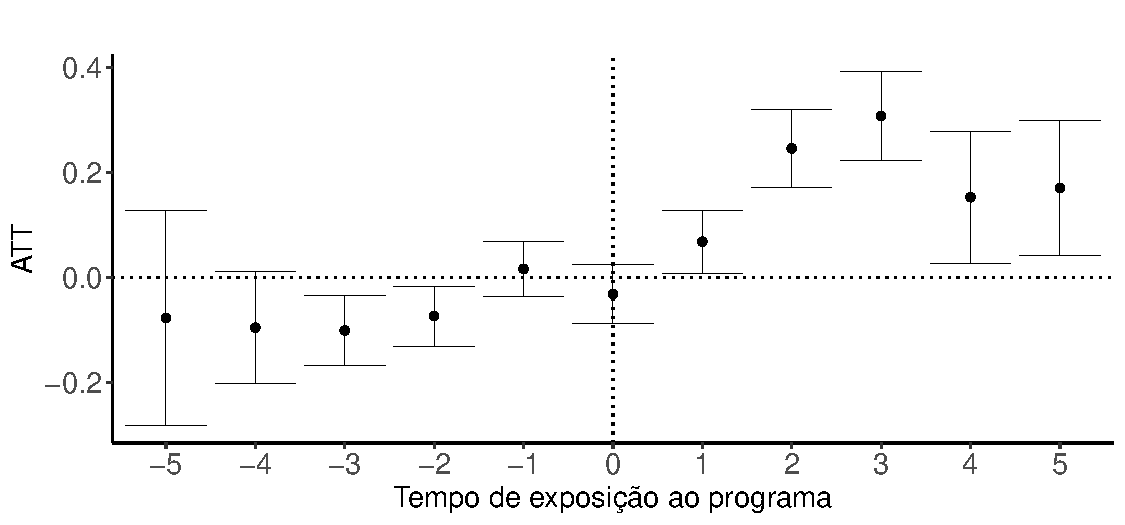
\includegraphics[width=1\linewidth]{Charts/did_agg_matematica.pdf}  
  \caption{Matemática}
  \label{fig:efeito_matematica}
\end{subfigure}
\begin{subfigure}{.5\textwidth}
  \centering
  % include second image
  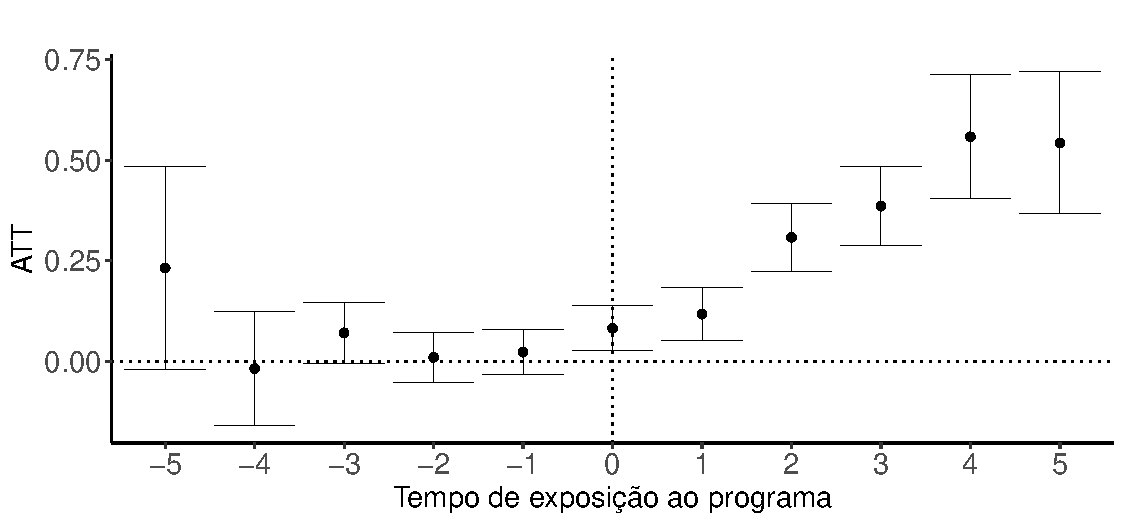
\includegraphics[width=1\linewidth]{Charts/did_agg_linguagem.pdf}  
  \caption{Linguagens}
  \label{fig:efeito_linguagem}
\end{subfigure}\newline

\begin{subfigure}{.5\textwidth}
  \centering
  % include third image
  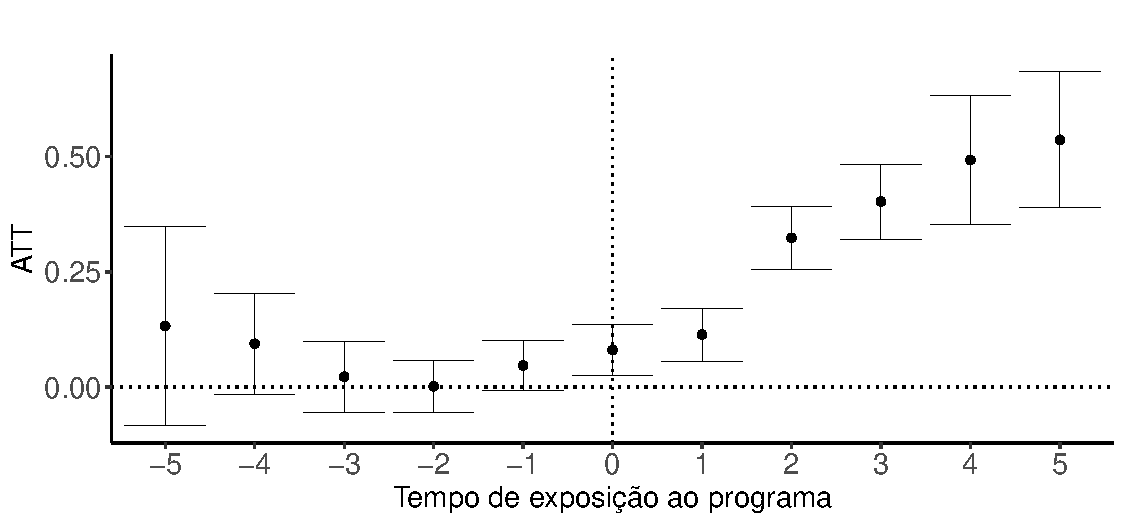
\includegraphics[width=1\linewidth]{Charts/did_agg_ciencias.pdf}  
  \caption{Ciências Naturais}
  \label{fig:efeito_ciencias}
\end{subfigure}
\begin{subfigure}{.5\textwidth}
  \centering
  % include fourth image
  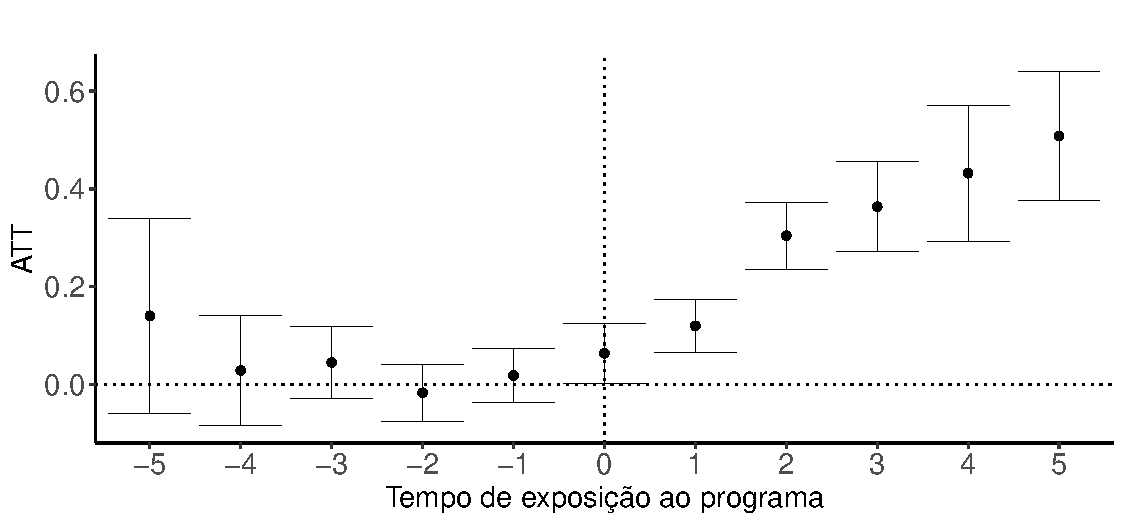
\includegraphics[width=1\linewidth]{Charts/did_agg_humanas.pdf}  
  \caption{Ciências Humanas}
  \label{fig:efeito_humanas}
\end{subfigure}
\begin{subfigure}{.5\textwidth}
  \centering
  % include first image
  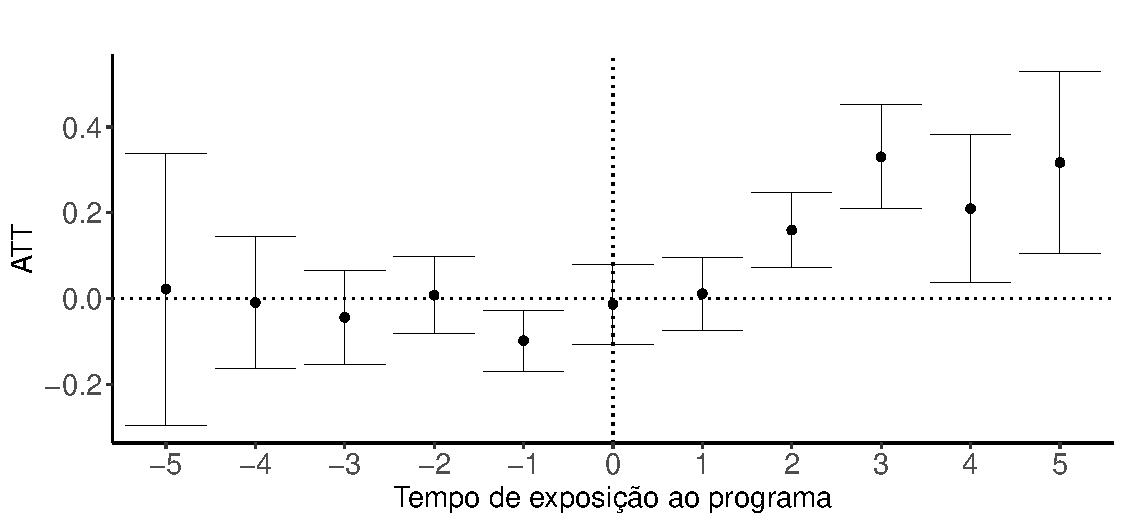
\includegraphics[width=1\linewidth]{Charts/did_agg_redacao.pdf}  
  \caption{Redação}
  \label{fig:efeito_redacao}
\end{subfigure}
\begin{subfigure}{.5\textwidth}
  \centering
  % include fourth image
  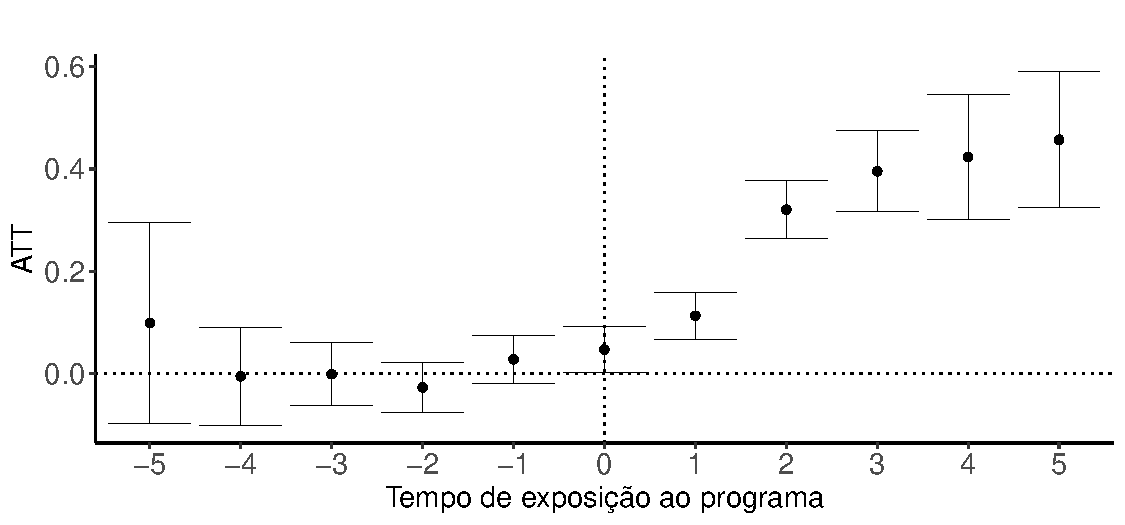
\includegraphics[width=1\linewidth]{Charts/did_agg_objetiva.pdf}  
  \caption{Geral em Objetivas}
  \label{fig:efeito_objetiva}
\end{subfigure}
\legend{Fontes: Elaboração própria, 2024}
\label{fig:efeito_agg_objetivas}
\end{figure}

\begin{figure}[b]
\caption{Efeito agregado sobre indicadores educacionais}
\begin{subfigure}{.5\textwidth}
  \centering
  % include first image
  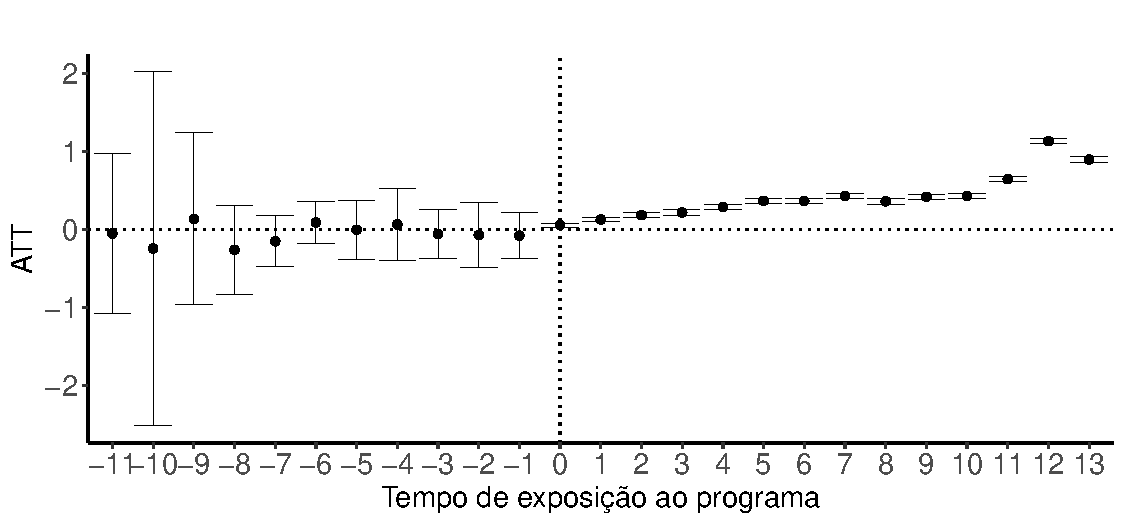
\includegraphics[width=1\linewidth]{Charts/did_agg_aprovacao.pdf}  
  \caption{Aprovação}
  \label{fig:efeito_aprovacao}
\end{subfigure}
\begin{subfigure}{.5\textwidth}
  \centering
  % include second image
  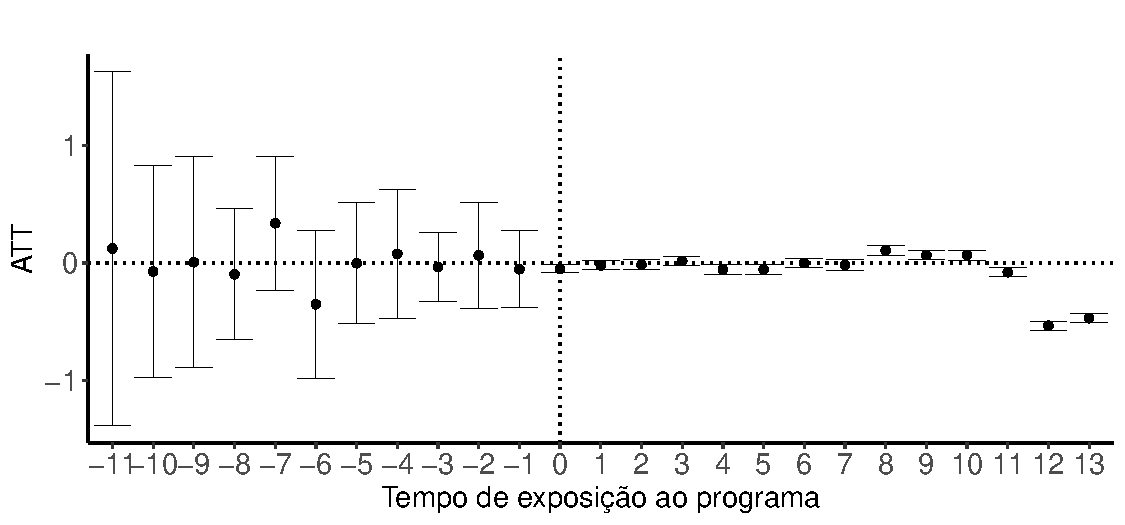
\includegraphics[width=1\linewidth]{Charts/did_agg_reprovacao.pdf}  
  \caption{Reprovação}
  \label{fig:efeito_reprovacao}
\end{subfigure}\newline

\begin{subfigure}{.5\textwidth}
  \centering
  % include third image
  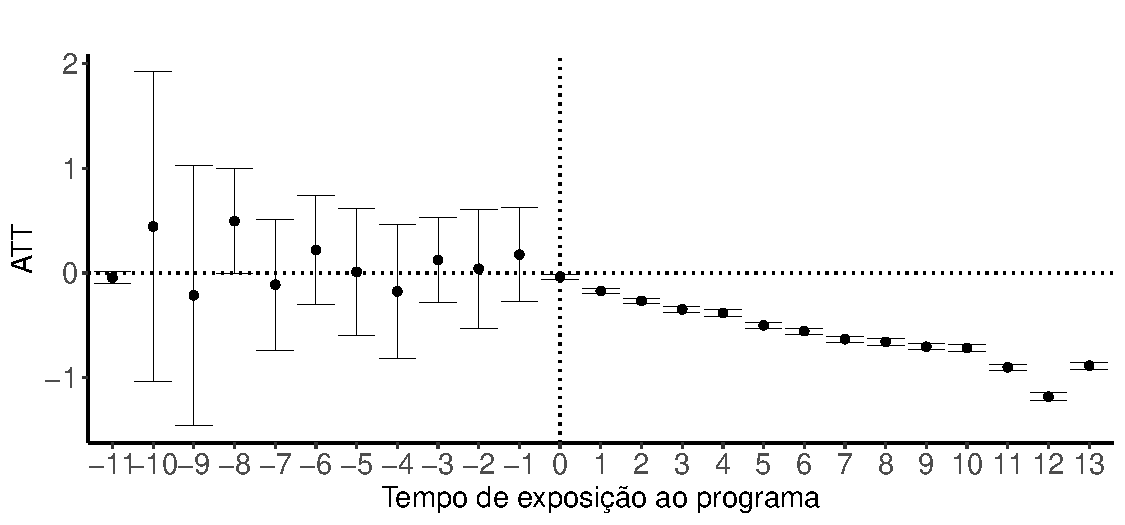
\includegraphics[width=1\linewidth]{Charts/did_agg_abandono.pdf}  
  \caption{Abandono}
  \label{fig:efeito_abandono}
\end{subfigure}
\begin{subfigure}{.5\textwidth}
  \centering
  % include fourth image
  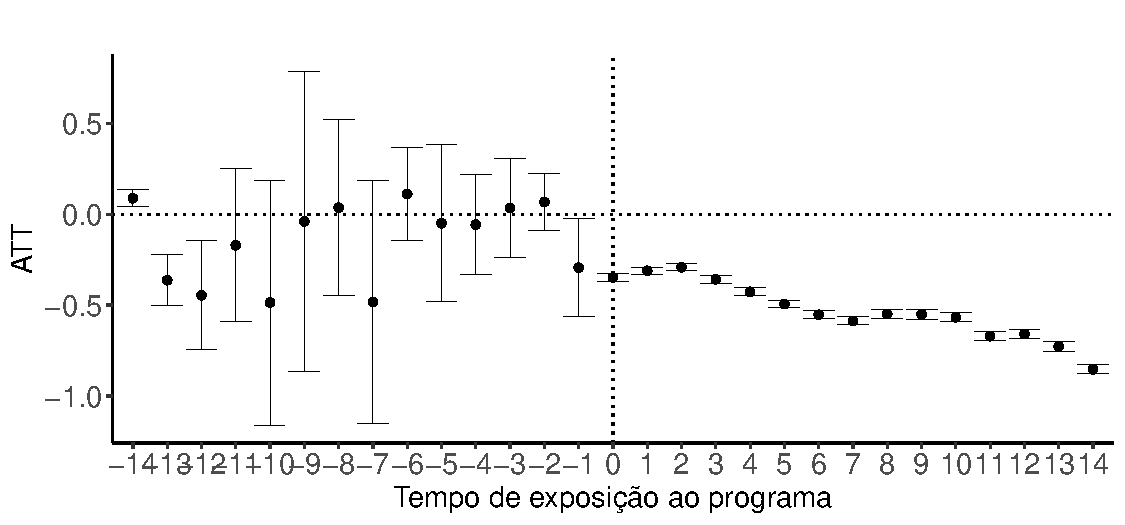
\includegraphics[width=1\linewidth]{Charts/did_agg_distorcao.pdf}  
  \caption{Distorção}
  \label{fig:efeito_distorcao}
\end{subfigure}

\legend{Fontes: Elaboração própria, 2024}
\label{fig:efeito_agg_indicadores}
\end{figure}

% PARTE DA PREPARAÇÃO DA PESQUISA
% ----------------------------------------------------------
%\part{Preparação da pesquisa}
%\input{cap02}
%

% PARTE DOS REFERENCIAIS TEÓRICOS
% ----------------------------------------------------------
%\part{Referenciais teóricos}
%\input{cap03}

% PARTE DOS RESULTADOS
% ----------------------------------------------------------
%\part{Resultados}
%\input{cap05}

% Finaliza a parte no bookmark do PDF
% para que se inicie o bookmark na raiz
% e adiciona espaço de parte no Sumário
% ----------------------------------------------------------
\phantompart

% ---
% Conclusão (outro exemplo de capítulo sem numeração e presente no sumário)
% ---
\chapter*[Conclusão]{Conclusão}
\addcontentsline{toc}{chapter}{CONCLUSÃO}
Este trabalho teve como objetivo estimar o impacto do programa de Ensino Médio Integral sobre um conjunto de indicadores escolares composto pela nota de estudantes nas provas do Exame Nacional do Ensino Médio (Enem) e para taxa de aprovação, reprovação, abandono e distorção idade-série para as escolas participantes do Censo Escolar do Instituto Nacional de Estudos e Pesquisas Educacionais Anísio Teixeira (INEP). 

Tendo como objetivo alcançar a meta 6 do Plano Nacional de Educação (PNE), o programa Ensino Médio Integral além de implementar a transição da jornada escolar de 4 horas diárias para 9 horas diárias, também implementa novas práticas pedagógicas e administrativas para as escolas participantes. 
Os resultados encontrados na literatura internacional e nacional para a implementação de programas de ensino integral não apresentam um consenso. Em especial, para o programa em análise aqui, vemos que a literatura traz efeitos em sentidos de melhora para as variáveis de interesse.

Entretanto, tal literatura baseia-se em métodos empíricos que não levam em consideração a possibilidade de entrada de escolas no programa ao longo do período de análise, trazendo viés para o estimador do efeito de tratamento sobre os tratados do método \textit{two-way fixed effect differences in differences}, amplamente utilizado na literatura. Como forma de correção propomos a adoção do método de \textit{staggered difference in differences} para avaliar se o programa trouxe resultados positivos para as escolas.

O método nos permite verificar o efeito agregados entre tratados e nunca tratados e como esse efeito evolui ao longo do tempo de exposição ao programa. Para as variáveis de nota observamos um aumento de aproximadamente 0,29 desvios padrões para a variável de nota geral em objetivas, 0,33 desvios para nota em linguagens, 0,32 desvios para nota em ciências naturais e 0,30 desvios para nota em ciências humanas. Ademais, para este conjunto de variáveis observamos  ganhos de nota ao longo do tempo de exposição ao programa. Este resultado nos leva a evidências de ganhos relevantes para alunos das escolas expostas a mais tempo ao programa, resultados os quais podem trazer ganhos relevantes em termos classificatórios em vestibulares que aceitam a nota do ENEM. Quando comparamos estes resultados com a literatura, observamos efeitos menores, mas com efeitos de tempo de exposição com tendência mais pronunciada. Já para o conjunto de indicadores educacionais observamos que os resultados de maior magnitude estão relacionados à taxa de aprovação,que apresenta um acréscimo de 0,42 desvios padrões e à taxa de abandono, que registra uma diminuição de 0,57 desvios. Tais variáveis possuem tendências positivas ao longo do tempo de exposição, mas sendo estes menores que os encontrados na literatura.






% ---
%\input{cap06}

% ELEMENTOS PÓS-TEXTUAIS
% ----------------------------------------------------------
\postextual

% Ajuste vertical do titulo de referencias no sumário
% ----------------------------------------------------------
\addtocontents{toc}{\vspace{-6pt}}

% Referências bibliográficas
% ----------------------------------------------------------
%\bibliography{referencias}

\begingroup

\printbibliography[heading=bay,notkeyword= {consulta}, notkeyword={npub-informal}]

\printbibliography [keyword= consulta, title = FONTES DE CONSULTA]
\endgroup

% ----------------------------------------------------------

% Ajuste vertical dos titulos dos capitulos postextuais
% ----------------------------------------------------------
\addtocontents{toc}{\vspace{4pt}}

% Glossário
% ----------------------------------------------------------
% Consulte o manual da classe abntex2 para orientações sobre o glossário.
%
%\glossary

% Apêndices
% ----------------------------------------------------------
\ifthenelse{\equal{\terApendice}{Sim}}
{% Apêndices
\begin{apendicesenv}
%
% Imprime uma página indicando o início dos apêndices
% \partapendices
\begin{landscape}

\chapter{Descrição das variáveis da base de dados}\label{apendice_descricao}


\begin{longtable}{cc}
% header and footer information
\caption{Principais variáveis da base de dados}\label{tab:descricao_base}

\\ \hline
Variável & Descrição\\
\hline
\endhead
\multicolumn{1}{l|}{Nota em matemática} &
  Média dos alunos da escola nos testes de matemática. \\
  \multicolumn{1}{l|}{Nota em linguagens} &
  Média dos alunos da escola nos testes de linguagem. \\
  \multicolumn{1}{l|}{Nota em ciências humanas} &
  Média dos alunos da escola nos testes de ciências humanas. \\
    \multicolumn{1}{l|}{Nota em ciências naturais} &
  Média dos alunos da escola nos testes de ciências naturais. \\
    \multicolumn{1}{l|}{Nota geral em provas objetivas} &
  Média dos alunos da escola nos testes de objetivos. \\
\multicolumn{1}{l|}{Nota redação}                       & Média dos alunos da escola no teste de escrita.                             \\
\multicolumn{1}{l|}{Taxa de aprovação}                  & Porcentagem de alunos na escola que foram aprovados.                        \\
\multicolumn{1}{l|}{Taxa de reprovação}                 & Porcentagem de alunos na escola que foram reprovados.                       \\
\multicolumn{1}{l|}{Taxa de abandono}                   & Porcentagem de alunos na escola que a abandonaram.                          \\
\multicolumn{1}{l|}{Distorção idade-série}              & Porcentagem de alunos na escola cuja idade é superior a ideal para a série. \\
\multicolumn{1}{l|}{Zona rural}                         & Escola na zona rural?                                                       \\
\multicolumn{1}{l|}{Diretoria}                    & Escola possui sala de diretor?                                              \\
\multicolumn{1}{l|}{Sala de leitura}                & Escola possui sala de leitura?                                          \\
\multicolumn{1}{l|}{Biblioteca}                         & Escola possui biblioteca?                                                   \\
\multicolumn{1}{l|}{Internet}                  & Escola possui acesso a internet?                                            \\
\multicolumn{1}{l|}{Laboratório de ciências}                         & Escola possui laboratório de ciências?                                                   \\
\multicolumn{1}{l|}{Quadra de esportes}                         & Escola possui quadra de esportes?                                                   \\

\multicolumn{1}{l|}{Coleta de lixo}          & Escola possui serviço de coleta de lixo?                                    \\
\multicolumn{1}{l|}{Água potável}                      & Escola possui acesso a rede de água?                                        \\
\multicolumn{1}{l|}{Esgoto}                    & Escola possui acesso a rede de esgoto?                                      \\
\multicolumn{1}{l|}{Eletricidade}              & Escola possui acesso a eletricidade?                                        \\
\multicolumn{1}{l|}{Número de alunos no ensino médio}   & Número total de alunos de ensino médio                                      \\
\multicolumn{1}{l|}{Número de mulheres no ensino médio} & Número total de mulheres no ensino médio                             \\
\multicolumn{1}{l|}{Número de alunos brancos no ensino médio}  & Número total de alunos brancos no ensino médio                   \\
\multicolumn{1}{l|}{Uso de transporte público no ensino médio}  & Número total alunos do ensino médio que usam transporte público                   \\
\multicolumn{1}{l|}{Mora com mais de seis pessoas}      & Porcentagem de alunos na escola que moram com mais de seis pessoas.         \\
\multicolumn{1}{l|}{Renda familiar maior que cinco salários mínimos} &
  Porcentagem de alunos na escola cuja renda familiar é superior ou igual a cinco salários mínimos. \\
\multicolumn{1}{l|}{Já procurou ou está a procura de trabalho} &
  Porcentagem de alunos na escola que já procuraram ou estão procurando emprego. \\
\multicolumn{1}{l|}{Ano de adoção do programa}          & Ano de entrada da escola no programa de ensino integral  \\ 
\hline
\end{longtable}
\legend{Fonte: Elaboração própria, 2024.} 
\end{landscape}

\chapter{Resultados Base}\label{apendice_resultados}

\begin{table}[htbp]
\caption{Resultados para nota em linguagens}
\centering
\begin{tabular}{cccccc}
\\ \hline
Tempo de Tratamento & Estimativa & Erro Padrão & IC [95\%] \\
\\ \hline
-5 & 0.2320 & 0.0961 & [-0.0236; 0.4877] \\
-4 & -0.0179 & 0.0513 & [-0.1544; 0.1186] \\
-3 & 0.0710 & 0.0271 & [-0.0011; 0.1431] \\
-2 & 0.0099 & 0.0222 & [-0.0493; 0.0691] \\
-1 & 0.0226 & 0.0210 & [-0.0332; 0.0784] \\
0 & 0.0819 & 0.0222 & [0.0230; 0.1409] \\
1 & 0.1169 & 0.0226 & [0.0567; 0.1771] \\
2 & 0.3079 & 0.0287 & [0.2317; 0.3841] \\
3 & 0.3855 & 0.0402 & [0.2787; 0.4924] \\
4 & 0.5579 & 0.0551 & [0.4115; 0.7044] \\
5 & 0.5429 & 0.0671 & [0.3645; 0.7212] \\
\\ \hline
\end{tabular}
\legend{Fonte: Elaboração própria, 2024.} 
\label{tab:resultados_linguagens}
\end{table}

\begin{table}[htbp]
\caption{Resultados para nota em redação}
\centering
\begin{tabular}{cccccc}
\\ \hline
Tempo de Tratamento & Estimativa & Erro Padrão & IC [95\%] \\
\\ \hline
-5 & 0.0216 & 0.1111 & [-0.2787; 0.3219] \\
-4 & -0.0095 & 0.0511 & [-0.1475; 0.1285] \\
-3 & -0.0442 & 0.0434 & [-0.1616; 0.0732] \\
-2 & 0.0075 & 0.0289 & [-0.0707; 0.0857] \\
-1 & -0.0984 & 0.0255 & [-0.1674; -0.0294] \\
0 & -0.0137 & 0.0342 & [-0.1062; 0.0788] \\
1 & 0.0110 & 0.0319 & [-0.0752; 0.0972] \\
2 & 0.1594 & 0.0324 & [0.0717; 0.2470] \\
3 & 0.3306 & 0.0389 & [0.2255; 0.4358] \\
4 & 0.2096 & 0.0547 & [0.0618; 0.3575] \\
5 & 0.3170 & 0.0681 & [0.1330; 0.5010] \\
\\ \hline
\end{tabular}
\legend{Fonte: Elaboração própria, 2024.} 
\label{tab:resultados_redacao}
\end{table}

\begin{table}[htbp]
\caption{Resultados para nota em matemática}
\centering
\begin{tabular}{cccccc}
\\ \hline
Tempo de Tratamento & Estimativa & Erro Padrão & IC [95\%] \\
\\ \hline
-5 & -0.0772 & 0.0670 & [-0.2524; 0.0981] \\
-4 & -0.0957 & 0.0357 & [-0.1892; -0.0021] \\
-3 & -0.1010 & 0.0248 & [-0.1658; -0.0362] \\
-2 & -0.0737 & 0.0192 & [-0.1240; -0.0234] \\
-1 & 0.0163 & 0.0162 & [-0.0260; 0.0587] \\
0 & -0.0318 & 0.0201 & [-0.0843; 0.0207] \\
1 & 0.0684 & 0.0222 & [0.0104; 0.1264] \\
2 & 0.2462 & 0.0290 & [0.1704; 0.3221] \\
3 & 0.3078 & 0.0315 & [0.2253; 0.3903] \\
4 & 0.1533 & 0.0473 & [0.0294; 0.2771] \\
5 & 0.1705 & 0.0437 & [0.0561; 0.2850] \\
\\ \hline
\end{tabular}
\legend{Fonte: Elaboração própria, 2024.} 
\label{tab:resultados_matematica}
\end{table}

\begin{table}[htbp]
\caption{Resultados para nota em ciências naturais}
\centering
\begin{tabular}{cccccc}
\\ \hline
Tempo de Tratamento & Estimativa & Erro Padrão & IC [95\%] \\
\\ \hline
-5 & 0.1330 & 0.0860 & [-0.1053; 0.3713] \\
-4 & 0.0940 & 0.0415 & [-0.0209; 0.2089] \\
-3 & 0.0226 & 0.0270 & [-0.0521; 0.0972] \\
-2 & 0.0016 & 0.0208 & [-0.0561; 0.0594] \\
-1 & 0.0468 & 0.0186 & [-0.0048; 0.0983] \\
0 & 0.0805 & 0.0199 & [0.0254; 0.1357] \\
1 & 0.1140 & 0.0207 & [0.0567; 0.1713] \\
2 & 0.3238 & 0.0236 & [0.2585; 0.3891] \\
3 & 0.4027 & 0.0328 & [0.3119; 0.4936] \\
4 & 0.4929 & 0.0448 & [0.3687; 0.6171] \\
5 & 0.5368 & 0.0554 & [0.3834; 0.6901] \\
\\ \hline
\end{tabular}
\legend{Fonte: Elaboração própria, 2024.} 
\label{tab:resultados_ciencias}
\end{table}

\begin{table}[htbp]
\caption{Resultados para nota em ciências humanas}
\centering
\begin{tabular}{cccccc}
\\ \hline
Tempo de Tratamento & Estimativa & Erro Padrão & IC [95\%] \\
\\ \hline
-5 & 0.1406 & 0.0802 & [-0.0814; 0.3625] \\
-4 & 0.0287 & 0.0380 & [-0.0765; 0.1340] \\
-3 & 0.0450 & 0.0253 & [-0.0249; 0.1149] \\
-2 & -0.0169 & 0.0213 & [-0.0758; 0.0419] \\
-1 & 0.0185 & 0.0193 & [-0.0348; 0.0717] \\
0 & 0.0640 & 0.0194 & [0.0103; 0.1177] \\
1 & 0.1198 & 0.0196 & [0.0657; 0.1740] \\
2 & 0.3043 & 0.0235 & [0.2394; 0.3693] \\
3 & 0.3637 & 0.0321 & [0.2750; 0.4524] \\
4 & 0.4320 & 0.0465 & [0.3035; 0.5606] \\
5 & 0.5078 & 0.0492 & [0.3716; 0.6440] \\
\\ \hline
\end{tabular}
\legend{Fonte: Elaboração própria, 2024.} 
\label{tab:resultados_humanas}
\end{table}

\begin{table}[htbp]
\caption{Resultados para nota geral em objetivas}
\centering
\begin{tabular}{cccccc}
\\ \hline
Tempo de Tratamento & Estimativa & Erro Padrão & IC [95\%] \\
\\ \hline
-5 & 0.0987 & 0.0729 & [-0.1018; 0.2991] \\
-4 & -0.0059 & 0.0369 & [-0.1074; 0.0957] \\
-3 & -0.0016 & 0.0228 & [-0.0644; 0.0611] \\
-2 & -0.0277 & 0.0186 & [-0.0789; 0.0236] \\
-1 & 0.0274 & 0.0153 & [-0.0146; 0.0695] \\
0 & 0.0466 & 0.0174 & [-0.0013; 0.0944] \\
1 & 0.1125 & 0.0190 & [0.0604; 0.1646] \\
2 & 0.3201 & 0.0217 & [0.2605; 0.3798] \\
3 & 0.3953 & 0.0289 & [0.3158; 0.4747] \\
4 & 0.4230 & 0.0437 & [0.3030; 0.5430] \\
5 & 0.4573 & 0.0508 & [0.3177; 0.5969] \\
\\ \hline
\end{tabular}
\legend{Fonte: Elaboração própria, 2024.} 
\label{tab:resultados_objetiva}
\end{table}

\begin{table}[htbp]
\caption{Resultados para taxa de abandono}  
\centering
\begin{tabular}{cccccc}
\\ \hline
Tempo de Tratamento & Estimativa & Erro Padrão & IC [95\%] \\
\\ \hline
-11 & -0.0458 & 0.0213 & [-0.1048; 0.0132] \\
-10 & 0.4443 & 0.5439 & [-1.0646; 1.9532] \\
-9 & -0.2137 & 0.4566 & [-1.4804; 1.0531] \\
-8 & 0.4961 & 0.1774 & [0.0039; 0.9883] \\
-7 & -0.1123 & 0.2225 & [-0.7296; 0.5049] \\
-6 & 0.2196 & 0.1961 & [-0.3244; 0.7635] \\
-5 & 0.0100 & 0.2335 & [-0.6378; 0.6578] \\
-4 & -0.1765 & 0.2318 & [-0.8197; 0.4666] \\
-3 & 0.1233 & 0.1500 & [-0.2926; 0.5393] \\
-2 & 0.0397 & 0.2155 & [-0.5580; 0.6375] \\
-1 & 0.1755 & 0.1740 & [-0.3072; 0.6581] \\
0 & -0.0353 & 0.0085 & [-0.0588; -0.0118] \\
1 & -0.1733 & 0.0083 & [-0.1964; -0.1501] \\
2 & -0.2673 & 0.0094 & [-0.2934; -0.2412] \\
3 & -0.3485 & 0.0106 & [-0.3779; -0.3191] \\
4 & -0.3832 & 0.0109 & [-0.4133; -0.3531] \\
5 & -0.5013 & 0.0106 & [-0.5307; -0.4719] \\
6 & -0.5562 & 0.0106 & [-0.5855; -0.5269] \\
7 & -0.6336 & 0.0101 & [-0.6616; -0.6056] \\
8 & -0.6592 & 0.0115 & [-0.6910; -0.6273] \\
9 & -0.7059 & 0.0107 & [-0.7354; -0.6763] \\
10 & -0.7176 & 0.0108 & [-0.7476; -0.6876] \\
11 & -0.9020 & 0.0108 & [-0.9319; -0.8720] \\
12 & -1.1834 & 0.0150 & [-1.2249; -1.1419] \\
13 & -0.8868 & 0.0115 & [-0.9188; -0.8548] \\
\\ \hline
\end{tabular}
\legend{Fonte: Elaboração própria, 2024.} 
\label{tab:resultados_abandono}
\end{table}

\begin{table}[htbp]
\caption{Resultados para taxa de reprovação}
\centering
\begin{tabular}{cccccc}
\\ \hline
Tempo de Tratamento & Estimativa & Erro Padrão & IC [95\%] \\
\\ \hline
-11 & 0.1231 & 0.5499 & [-2.0371; 2.2832] \\
-10 & -0.0726 & 0.3285 & [-1.3631; 1.2180] \\
-9 & 0.0060 & 0.5242 & [-2.0533; 2.0653] \\
-8 & -0.0970 & 0.2042 & [-0.8993; 0.7052] \\
-7 & 0.3381 & 0.2123 & [-0.4959; 1.1722] \\
-6 & -0.3523 & 0.2397 & [-1.2938; 0.5893] \\
-5 & -0.0024 & 0.1839 & [-0.7249; 0.7201] \\
-4 & 0.0770 & 0.1893 & [-0.6666; 0.8205] \\
-3 & -0.0335 & 0.1130 & [-0.4774; 0.4104] \\
-2 & 0.0653 & 0.1577 & [-0.5541; 0.6847] \\
-1 & -0.0535 & 0.1085 & [-0.4799; 0.3729] \\
0 & -0.0508 & 0.0136 & [-0.1042; 0.0026] \\
1 & -0.0210 & 0.0138 & [-0.0752; 0.0333] \\
2 & -0.0150 & 0.0142 & [-0.0709; 0.0408] \\
3 & 0.0169 & 0.0151 & [-0.0424; 0.0761] \\
4 & -0.0563 & 0.0155 & [-0.1173; 0.0047] \\
5 & -0.0567 & 0.0162 & [-0.1203; 0.0069] \\
6 & -0.0013 & 0.0154 & [-0.0619; 0.0593] \\
7 & -0.0186 & 0.0150 & [-0.0775; 0.0404] \\
8 & 0.1085 & 0.0163 & [0.0445; 0.1725] \\
9 & 0.0667 & 0.0153 & [0.0064; 0.1270] \\
10 & 0.0658 & 0.0149 & [0.0071; 0.1244] \\
11 & -0.0790 & 0.0146 & [-0.1362; -0.0218] \\
12 & -0.5344 & 0.0147 & [-0.5922; -0.4766] \\
13 & -0.4705 & 0.0159 & [-0.5330; -0.4080] \\
\\ \hline
\end{tabular}
\legend{Fonte: Elaboração própria, 2024.} 
\label{tab:resultados_reprovacao}
\end{table}


\begin{table}[htbp]
\caption{Resultados para taxa de aprovação}
\centering
\begin{tabular}{cccccc}
\\ \hline
Tempo de Tratamento & Estimativa & Erro Padrão & IC [95\%] \\
\\ \hline
-11 & -0.0519 & 0.3514 & [-1.0386; 0.9349] \\
-10 & -0.2430 & 0.5755 & [-1.8591; 1.3730] \\
-9 & 0.1362 & 0.1876 & [-0.3907; 0.6630] \\
-8 & -0.2608 & 0.2003 & [-0.8232; 0.3016] \\
-7 & -0.1515 & 0.1123 & [-0.4670; 0.1640] \\
-6 & 0.0905 & 0.1055 & [-0.2057; 0.3868] \\
-5 & -0.0049 & 0.1187 & [-0.3384; 0.3285] \\
-4 & 0.0645 & 0.1719 & [-0.4183; 0.5473] \\
-3 & -0.0586 & 0.1077 & [-0.3609; 0.2438] \\
-2 & -0.0696 & 0.1432 & [-0.4717; 0.3326] \\
-1 & -0.0795 & 0.1052 & [-0.3748; 0.2159] \\
0 & 0.0567 & 0.0095 & [0.0300; 0.0834] \\
1 & 0.1274 & 0.0107 & [0.0974; 0.1574] \\
2 & 0.1851 & 0.0105 & [0.1557; 0.2144] \\
3 & 0.2170 & 0.0111 & [0.1858; 0.2482] \\
4 & 0.2885 & 0.0112 & [0.2571; 0.3200] \\
5 & 0.3662 & 0.0111 & [0.3350; 0.3974] \\
6 & 0.3653 & 0.0119 & [0.3320; 0.3986] \\
7 & 0.4276 & 0.0125 & [0.3925; 0.4627] \\
8 & 0.3597 & 0.0117 & [0.3268; 0.3927] \\
9 & 0.4182 & 0.0110 & [0.3874; 0.4490] \\
10 & 0.4265 & 0.0125 & [0.3915; 0.4616] \\
11 & 0.6439 & 0.0104 & [0.6147; 0.6731] \\
12 & 1.1316 & 0.0128 & [1.0957; 1.1674] \\
13 & 0.8947 & 0.0119 & [0.8612; 0.9281] \\
\\ \hline
\end{tabular}
\legend{Fonte: Elaboração própria, 2024.} 
\label{tab:resultados_aprovacao}
\end{table}

\begin{table}[htbp]
\caption{Resultados para taxa de distorção}
\centering
\begin{tabular}{cccccc}
\\ \hline
Tempo de Tratamento & Estimativa & Erro Padrão & IC [95\%] \\
\\ \hline
-14 & 0.0871 & 0.1796 & [-0.3900; 0.5642] \\
-13 & -0.3634 & 0.0947 & [-0.6150; -0.1118] \\
-12 & -0.4464 & 0.1093 & [-0.7368; -0.1559] \\
-11 & -0.1718 & 0.1595 & [-0.5956; 0.2520] \\
-10 & -0.4864 & 0.2643 & [-1.1885; 0.2157] \\
-9 & -0.0402 & 0.2840 & [-0.7946; 0.7143] \\
-8 & 0.0352 & 0.1691 & [-0.4140; 0.4844] \\
-7 & -0.4829 & 0.2480 & [-1.1419; 0.1760] \\
-6 & 0.1109 & 0.1015 & [-0.1586; 0.3805] \\
-5 & -0.0499 & 0.1701 & [-0.5017; 0.4019] \\
-4 & -0.0573 & 0.0974 & [-0.3161; 0.2015] \\
-3 & 0.0335 & 0.1116 & [-0.2631; 0.3300] \\
-2 & 0.0665 & 0.0656 & [-0.1076; 0.2407] \\
-1 & -0.2941 & 0.0993 & [-0.5578; -0.0305] \\
0 & -0.3481 & 0.0065 & [-0.3654; -0.3307] \\
1 & -0.3112 & 0.0067 & [-0.3290; -0.2934] \\
2 & -0.2918 & 0.0075 & [-0.3117; -0.2720] \\
3 & -0.3585 & 0.0076 & [-0.3787; -0.3383] \\
4 & -0.4270 & 0.0073 & [-0.4463; -0.4076] \\
5 & -0.4944 & 0.0073 & [-0.5138; -0.4750] \\
6 & -0.5532 & 0.0081 & [-0.5747; -0.5316] \\
7 & -0.5867 & 0.0091 & [-0.6110; -0.5625] \\
8 & -0.5493 & 0.0087 & [-0.5723; -0.5263] \\
9 & -0.5505 & 0.0089 & [-0.5741; -0.5270] \\
10 & -0.5675 & 0.0091 & [-0.5917; -0.5432] \\
11 & -0.6714 & 0.0094 & [-0.6964; -0.6464] \\
12 & -0.6587 & 0.0100 & [-0.6854; -0.6321] \\
13 & -0.7263 & 0.0094 & [-0.7512; -0.7014] \\
14 & -0.8533 & 0.0095 & [-0.8785; -0.8281] \\
\\ \hline
\end{tabular}
\legend{Fonte: Elaboração própria, 2024.} 
\label{tab:resultados_distorcao}
\end{table}
\end{apendicesenv}
}
{}

% Anexos
% ----------------------------------------------------------
\ifthenelse{\equal{\terAnexo}{Sim}}{
\begin{anexosenv}

        % Numeração arábica para os apêndices
        % --------------------------------------------------
        \renewcommand{\thechapter}{\arabic{chapter}}
        % --- Imprime uma página indicando o início dos anexos
        % \partanexos

        % Existem várias formas de se colocar anexos.
        % O exemplo abaixo coloca 2 anexos denominados de 
        % TABELA DE VALORES e GRÁFICOS DE BALANCEMANTO:
        % ---
        % --- insere um capítulo que é tratado como um anexo
        %\chapter{TABELAS DE VALORES}
        % 
        %\lipsum[31] % gera um parágrafo
        %
        % --- insere um capítulo que é tratado como um anexo
        %\chapter{GRÁFICOS DE BALANCEAMENTO}
        % 
        %\lipsum[32] % gera um parágrafo

        % --- Insere o texto do arquivo ax01.tex
        % 
        % --- O conteúdo do arquivo pode ser vários anexos ou um único anexo.
        %     A vantagem de se utilizar este procedimento é de suprimi-lo
        %     das compilações enquanto se processa o resto do documento.

            % --- insere um capítulo que é tratado como um apêndice
   \chapter{anexando ESCOLHA DO MATERIAL}
    
   \lipsum[30] % gera um parágrafo
    \section*{anexando testes secao}
    

\chapter{anexando ESCOLHA DO MATERIAL DE IMPRESSÃO}
    
   \lipsum[32] % gera um parágrafo
 
\end{anexosenv}}{}

% INDICE REMISSIVO
%---------------------------------------------------------------------
\ifthenelse{\equal{\terIndiceR}{Sim}}{
\phantompart
\printindex
}{}

\end{document}
